\documentclass[a4paper,12pt]{article}
\usepackage[T1]{fontenc}
\usepackage[utf8]{inputenc}
\usepackage{lmodern}
\usepackage{hyperref}
\usepackage{graphicx}
\usepackage{booktabs}
\usepackage{listings}
\usepackage{xcolor}
\usepackage{geometry}
\usepackage{enumitem}
\usepackage{caption}
\usepackage{pgf-umlsd}
\usepackage{float}

\geometry{margin=2.5cm}

\lstset{
  basicstyle=\ttfamily\small,
  breaklines=true,
  frame=single,
  keywordstyle=\color{blue}\bfseries,
  commentstyle=\color{green!50!black},
  stringstyle=\color{red!70!black},
  numbers=left,
  numberstyle=\tiny,
  tabsize=2,
}

\title{\textbf{EvenToNight}\\
Distributed Systems - Final Report}
\author{
  Alfonsi Alice (alice.alfonsi2@studio.unibo.it)\\
  Bravetti Federico (federico.bravetti2@studio.unibo.it)\\
  Brini Tommaso (tommaso.brini@studio.unibo.it)
}
\date{March 2026}

\begin{document}

\maketitle

\begin{abstract}
The project consists of the design and development of a distributed digital platform called \textbf{EvenToNight}, aimed at connecting organizations that promote social events with users interested in discovering and participating in them. The platform, accessible at \url{https://eventonight.site/}, can be used either as a guest or through a registered account that provides additional functionalities.

From a technical perspective, EvenToNight has been designed as a distributed system based on a microservices architecture, supporting modularity, scalability and the independent management of application components.

This architectural choice enables horizontal and autonomous scaling of the various system components, allowing the platform to handle a large number of users concurrently. Furthermore, the distributed architecture ensures reliable data persistence, availability and openness, thereby facilitating future extensions and adaptation to evolving requirements.

Overall, the project represents a practical application of distributed systems principles within the context of a realistic web-based platform.
\end{abstract}

\tableofcontents
\newpage

\section{Goals of the Project}
The main goals of the project are:

\begin{enumerate}
  \item \textbf{Create a digital platform for social events}: provide a platform for exploring, discovering social events and interacting with other users.
  \item \textbf{Support both public access and extended functionalities for registered users}: allow public browsing of events while offering additional functionalities for registered users and organizations.
  \item \textbf{Promote interaction between users and organizations}: enable users and organizations to communicate and collaborate on the platform.
  \item \textbf{Increase visibility and credibility of organizations}: enhance organizations' reputation through active community engagement.
  \item \textbf{Ensure system availability and scalability}: design the platform to handle distributed operations efficiently while maintaining responsiveness.
  \item \textbf{Guarantee transparency and coherence in the distributed architecture}: ensure users perceive the platform as a reliable and consistent system, even if it is implemented as a distributed architecture.
  \item \textbf{Enable future extensibility and adaptability}: design the system to easily incorporate new features, services or integrations without major changes.
\end{enumerate}

\subsection{Usage Scenarios}

This section illustrates the typical interactions between the target users of the platform and the system itself. EvenToNight has been conceived for three types of users: unregistered users, registered users and users registered as organizations.

The use case diagram in fig.~\ref{fig:case-diagram} summarizes the main interactions of these three user types with the platform.

\begin{figure}[H]
  \centering
  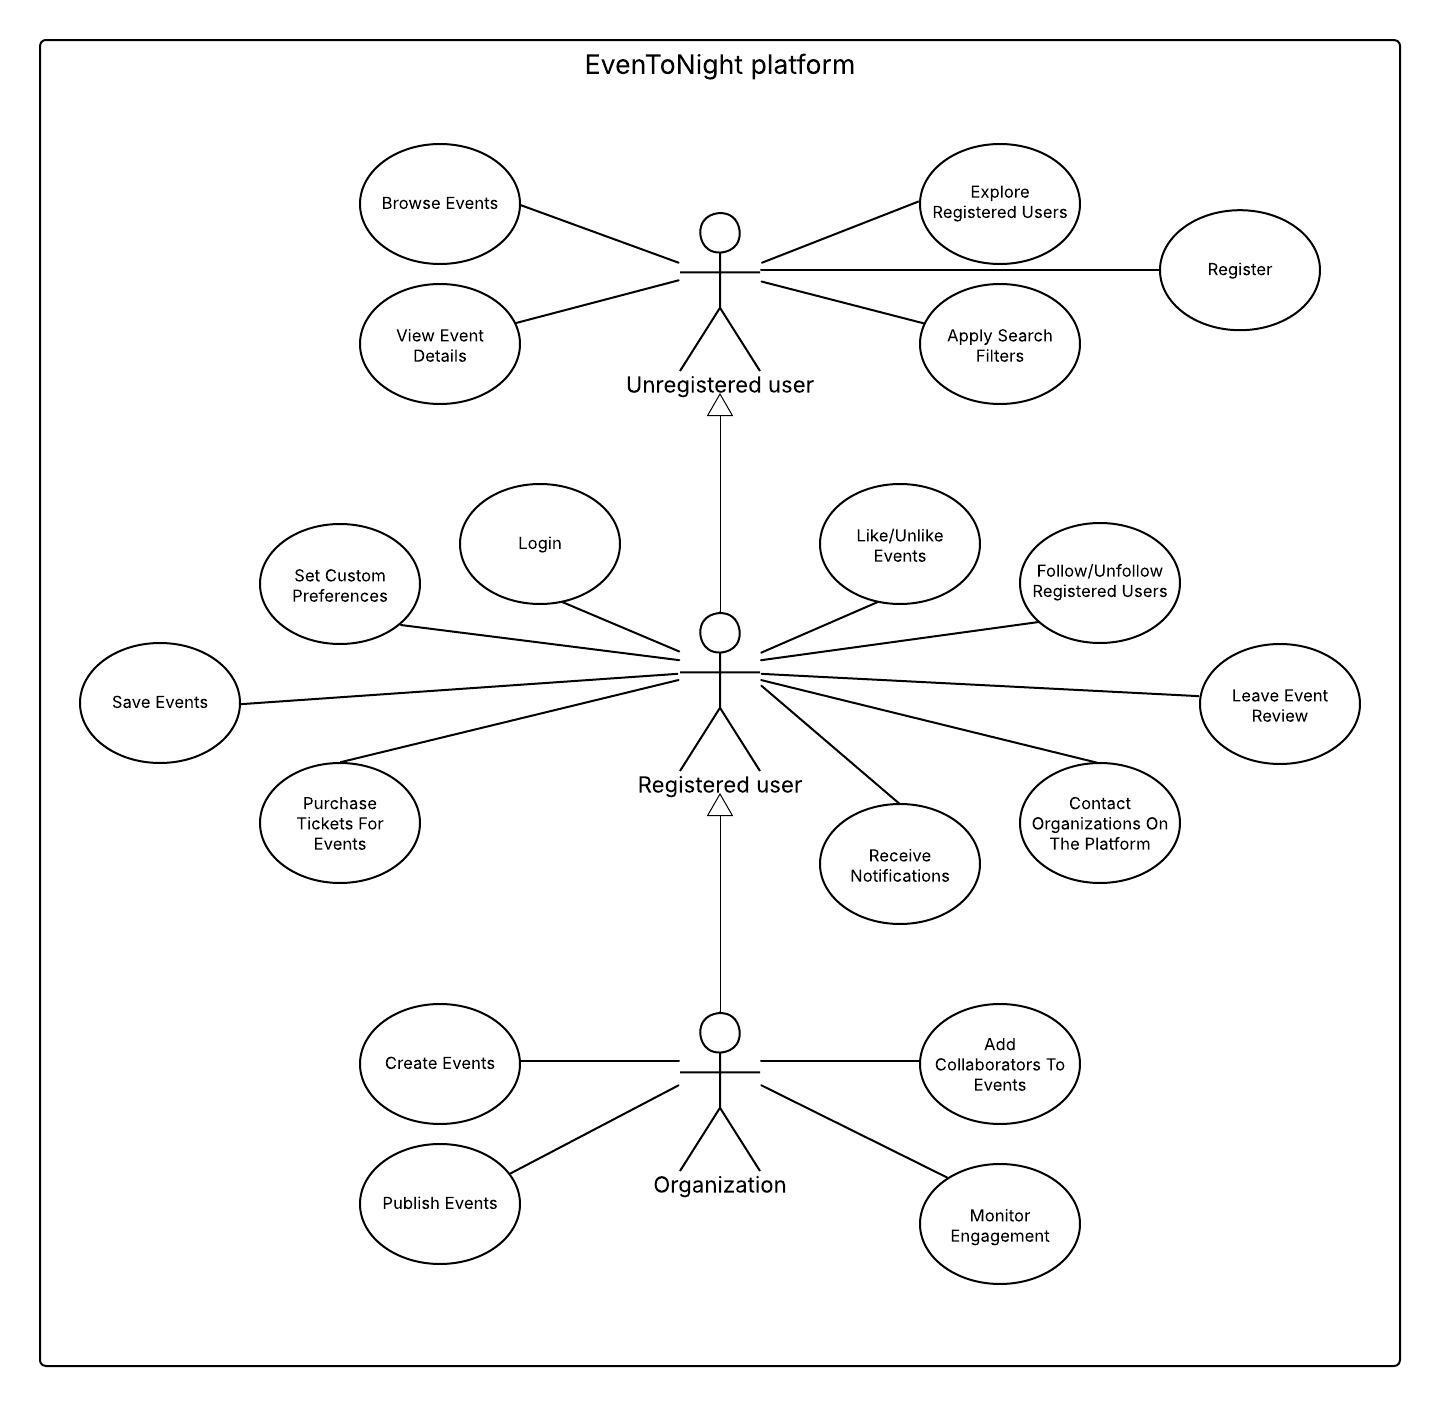
\includegraphics[width=\textwidth]{../public/case_diagram.jpeg}
  \caption{Use case diagram}
  \label{fig:case-diagram}
\end{figure}

\paragraph{Usage scenario: Browsing and filtering events as an unregistered user.}
\begin{itemize}
  \item \textbf{Actor}: Unregistered user.
  \item \textbf{Objective}: Explore events according to location and gather information without registering an account.
  \item \textbf{Main flow}:
    \begin{enumerate}
      \item The user browses the list of upcoming events.
      \item The user views event details, including poster, description, time and location.
      \item The user applies filters to find events nearby.
      \item The user searches for users registered on the platform.
    \end{enumerate}
  \item \textbf{Outcome}: The user accesses all event information without providing personal data and discovers other platform users.
\end{itemize}

\paragraph{Usage scenario: Personalized event discovery, ticket purchase and post-event review as a registered user.}
\begin{itemize}
  \item \textbf{Actor}: Registered user.
  \item \textbf{Objective}: Discover events based on personal preferences, evaluate them and purchase tickets.
  \item \textbf{Main flow}:
    \begin{enumerate}
      \item The user logs in to the EvenToNight platform.
      \item The user navigates their personalized event feed based on specified interests.
      \item The user selects an event and reads reviews on the organization's page.
      \item The user purchases tickets for the event.
    \end{enumerate}
  \item \textbf{Outcome}: The user quickly finds matching events, evaluates the organization's reliability and the purchased ticket appears on the user's personal page and can be downloaded.
  \item \textbf{Post-event action}: After attending the event, the user leaves a review on the organization's page.
\end{itemize}

\paragraph{Usage scenario: Saving events and contacting organizations as a registered user.}
\begin{itemize}
  \item \textbf{Actor}: Registered user.
  \item \textbf{Objective}: Navigate the platform, save events and contact organizations via a customized interface.
  \item \textbf{Main flow}:
    \begin{enumerate}
      \item The user logs in and navigates the platform with saved language and appearance settings.
      \item The user selects an event and saves it to their personal list.
      \item The user contacts the organization to request additional information.
    \end{enumerate}
  \item \textbf{Outcome}: Selected events are stored in the user's personal list and the user can communicate with the organization through the platform.
\end{itemize}

\paragraph{Usage scenario: Publication of events and monitoring engagement as an organization.}
\begin{itemize}
  \item \textbf{Actor}: Organization.
  \item \textbf{Objective}: Publish events and monitor user engagement.
  \item \textbf{Main flow}:
    \begin{enumerate}
      \item The user logs in and creates an event as a draft.
      \item The user adds a collaborating organization to the event.
      \item The user publishes the event.
    \end{enumerate}
  \item \textbf{Outcome}: The event is successfully published and the organization receives notifications about new followers and event likes.
\end{itemize}

\subsection{Definition of Done}

The project is considered \textit{done} when the following criteria are met:

\begin{enumerate}
  \item \textbf{Requirements fulfilled.} All main functionalities of the platform are implemented and all business and non-functional requirements are satisfied.
  \item \textbf{Testing completed.} Unit and integration tests for all services pass successfully. All API endpoints have been verified using Swagger/OpenAPI.
  \item \textbf{Deploy ready.} All services are containerized and managed via Docker Compose. The simulated distributed environment demonstrates service isolation and internal networking.
  \item \textbf{Documentation updated.} API documentation, architectural diagrams and project documentation are complete, consistent and up to date.
\end{enumerate}

\newpage
\section{Background and Link to the Theory}

In the following are presented the main distributed system concepts related to this project, the main architectural and interaction patterns, and the technologies used.

\subsection{Distributed Systems Fundamentals}

\textbf{CAP theorem} states that a distributed system can guarantee at most two of three properties simultaneously: \textit{Consistency} (all nodes see the same data at the same time), \textit{Availability} (every request receives a response) and \textit{Partition tolerance} (the system continues operating despite network partitions). Since partition tolerance is non-negotiable in a real network, systems must choose between consistency and availability under a partition. Systems that prioritise availability accept that replicas may temporarily diverge, relying instead on \textit{eventual consistency}.

\textbf{Eventual consistency} is a consistency model in which, in the absence of new updates, all replicas of a data item will converge to the same value over time. It trades immediate cross-service consistency for higher availability and lower coupling, accepting that different parts of the system may temporarily observe slightly different states.

\textbf{FLP impossibility result} (Fischer, Lynch, Paterson) proves that in a fully asynchronous distributed system, consensus cannot be guaranteed if even a single process may fail. In practice this means failure detection is impossible without some notion of time: a slow process is indistinguishable from a crashed one. \textbf{Timeouts} are the practical solution and motivate \textbf{exponential backoff} in reconnection logic, spacing out retries to avoid overwhelming a recovering dependency.

\textbf{Availability} is the degree to which a system is operational and responsive when needed. \textbf{High availability (HA)} extends this by designing the system to minimise downtime through redundancy and automatic failover.

\textbf{At-least-once delivery} is a message delivery guarantee where the broker ensures a message is delivered to the consumer at least once, but may deliver it more than once in the event of failures or retries. Consumers must therefore be designed to tolerate duplicate messages.

\textbf{Idempotency} is the property of an operation whereby applying it multiple times produces the same result as applying it once. In distributed systems, idempotent message handlers are the standard mitigation for at-least-once delivery semantics.

\subsection{Architectural Styles}

\textbf{Microservices} decompose an application into small, independently deployable services, each responsible for a single bounded context. Combined with the \textbf{database-per-service} pattern, each service owns its data store exclusively, preventing coupling at the persistence layer and allowing schemas to evolve independently.

\textbf{Event-Driven Architecture} decouples producers and consumers of events, avoiding direct synchronous calls. This reduces temporal coupling, improves scalability and allows new consumers to be added without changing existing producers.

\textbf{Domain-Driven Design (DDD)} provides the modeling vocabulary: a domain is partitioned into \textit{bounded contexts}, each with its own ubiquitous language. Within a context, \textit{aggregates} enforce business invariants, \textit{value objects} represent immutable concepts and \textit{domain events} describe state changes that other contexts may react to.

\textbf{Clean Architecture} organises a service's codebase into concentric layers (domain, application, infrastructure, presentation) with a strict inward dependency rule: outer layers depend on inner ones, never the reverse. This keeps domain logic framework-agnostic and independently testable.

\textbf{CQRS (Command Query Responsibility Segregation)} separates write operations (commands) from read operations (queries) at the application layer, assigning each to a dedicated handler. This makes individual operations smaller and more focused and opens the door to independent scaling of read and write paths.

\subsection{Interaction Patterns}

\textbf{REST over HTTP} is the standard synchronous request/response pattern: the client sends a request and blocks until the server replies. Suitable for operations that require an immediate result.

\textbf{AMQP (message broker)} enables asynchronous, decoupled communication. A producer publishes a message to an exchange; the broker routes it to bound queues; consumers process it independently. A \textit{topic exchange} routes messages by routing key pattern, allowing fine-grained subscriptions. \textit{Quorum queues} replicate messages across cluster nodes for durability and availability.

\textbf{WebSocket} provides a persistent, full-duplex channel between client and server, enabling server-initiated push without polling.

\textbf{Webhooks} allow external systems to push events into the application via HTTP callbacks, triggered by events on the provider's side.

\textbf{Transactional outbox} ensures reliable event publishing: the domain event is written to an outbox table in the same database transaction as the state change; a relay process reads from the outbox and forwards messages to the broker, retrying until success. This decouples message publishing from broker availability.

\textbf{Saga} coordinates a multi-step operation across services without a distributed transaction. Each step has a compensating action that can undo its effect if a later step fails.

\subsection{Software Frameworks and Technologies}

\begin{table}[H]
  \centering
  \begin{tabular}{ll}
    \toprule
    \textbf{Technology} & \textbf{Role} \\
    \midrule
    Docker / Compose / Swarm & Containerisation and orchestration \\
    Traefik & API gateway, reverse proxy, load balancer, rate limiter \\
    Cloudflare + cloudflared & DNS, TLS termination, encrypted inbound tunnel \\
    RabbitMQ & AMQP message broker \\
    MongoDB & Document store (per-service) \\
    PostgreSQL & Relational store (Keycloak) \\
    MinIO & S3-compatible object storage \\
    Keycloak & Identity provider, JWT issuance \\
    Stripe & Third-party payment provider \\
    NestJS & Node.js framework (structured modules, DI) \\
    Node.js + Express & Minimal HTTP server runtime \\
    Scala 3 + Cask & Functional backend services \\
    Vue 3 + Vite & Single-page application frontend \\
    Socket.IO & WebSocket abstraction with Redis pub/sub adapter \\
    \bottomrule
  \end{tabular}
  \caption{Software frameworks and technologies}
  \label{tab:technologies}
\end{table}

\newpage
\section{Requirements Analysis}

\subsection{Requirements List}

The main requirements that the application must meet are listed below.

\subsubsection{Business Requirements}

\begin{itemize}
  \item The platform allows organizations to create and publish posts related to the events they promote.
  \item The platform allows users to discover events based on their location and interests.
  \item The platform enables online ticket sales for events, allowing organizations to monetize them.
\end{itemize}

\subsubsection{Functional Requirements}

\noindent\textbf{Types of users supported by the system:}
\begin{itemize}
  \item \textbf{Unregistered users}, who can explore the platform.
  \item \textbf{Registered users}, who can access features reserved for authenticated users.
  \item \textbf{Users registered as an organization}, who can access all platform features and additionally create and publish events and manage ticketing.
\end{itemize}

\noindent\textbf{Functional requirements for all users:}
\begin{itemize}
  \item View the Home screen, including interaction modes such as searching for events, viewing popular events, upcoming events and latest additions.
  \item View all events published on the platform and all registered users from the Explore screen, applying search filters.
\end{itemize}

\noindent\textbf{Functional requirements for registered users:}
\begin{itemize}
  \item Receive a personalized event feed based on specified interests.
  \item Like and unlike events.
  \item Follow and unfollow other registered users.
  \item Purchase tickets for events.
  \item Leave a review after attending an event.
  \item Contact organizations directly within the platform to request support.
  \item Receive notifications about:
    \begin{itemize}
      \item new followers
      \item new events published by followed organizations
      \item new messages
    \end{itemize}
\end{itemize}

\noindent\textbf{Functional requirements for users registered as an organization:}
\begin{itemize}
  \item Create events, choosing whether to make them public or save them as drafts.
  \item Specify collaborators when creating events.
  \item Receive notifications about likes and reviews on their own events.
\end{itemize}

\subsubsection{Non-Functional Requirements}

\begin{itemize}
  \item \textbf{Availability}: every request sent to a non-failing node in the system must receive a response.
  \item \textbf{Reliability}: the system must operate correctly over time, minimizing the occurrence of faults.
  \item \textbf{Fault Tolerance}: the system must tolerate failures of individual services (i.e. containerized microservices) without affecting the overall platform operation.
  \item \textbf{Security}: the system requires user authentication and enforces authorization to access resources according to defined rules. In addition, to ensure password confidentiality, only a secure hash of each user's password will be stored.
  \item \textbf{Robustness}: the system must handle incorrect inputs, providing consistent error messages without compromising system stability.
  \item \textbf{Scalability}: the system must be able to handle increasing loads by adding new resources, without degrading performance.
  \item \textbf{Extensibility}: the system must support easy customization and the addition of new functionalities.
  \item \textbf{Maintainability}: the system must be easy to maintain with respect to the addition of new features and system updates. This is supported by well-structured and well-documented code.
  \item \textbf{Accessibility}: the system's graphical interface must be accessible, supporting standard accessibility guidelines.
  \item \textbf{Portability}: the system must be responsive and adapt to different screen sizes and devices, including PCs, tablets and smartphones.
  \item \textbf{Deployability}: the system must automatically update to the latest release version.
  \item \textbf{Architectural Constraint}: the system must be developed following a microservices architecture.
\end{itemize}

\subsection{Top-Down Analysis}

\subsubsection{Architectural Styles}

Starting from the identified requirements, an \textbf{event-based architecture} was selected to design the distributed platform.

This architectural style was chosen because it addresses several non-functional requirements of the system. In particular, the following architectural properties directly contribute to satisfying the system's non-functional requirements:

\begin{itemize}
  \item \textbf{Referential and spatial decoupling}: producers and consumers do not reference or depend on each other's location. This supports extensibility, allowing new services to be added without modifying existing components.
  \item \textbf{Temporal decoupling}: events are stored in a persistent event space until consumers are able to process them. This ensures that producer services remain responsive even if consumer services are temporarily unavailable, supporting fault tolerance and availability. In addition, this storage smooths load peaks by decoupling producer and consumer execution timing and it supports extensibility and horizontal scalability by allowing the addition of multiple consumer instances.
  \item \textbf{Loosely coupled services}: producers publish events without waiting for consumers to respond and consumers process events independently. This independence supports fault tolerance, maintainability and extensibility, as temporary service failures or modifications do not affect other components and the addition of new functionalities and service updates is simplified.
\end{itemize}

At the system boundary level, the platform also follows a \textbf{layered architecture}:

\begin{itemize}
  \item \textbf{Presentation layer}: the containerized frontend microservice, providing the user interface.
  \item \textbf{Application layer}: containerized backend microservices exposing REST APIs.
  \item \textbf{Data layer}: repositories interacting with databases for persistence.
\end{itemize}

The layered organization provides a high-level view of control flow in the distributed platform, highlighting the separation of concerns between user interface, business logic and data management.

\newpage
\section{Design}

The system has been designed following a microservices architectural style, where each service models a specific subdomain and exclusively owns its data.

The principal objective of the design phase has been to:
\begin{itemize}
  \item ensure service autonomy.
  \item separate services persistence management.
  \item guarantee scalability and fault isolation.
  \item preserve local consistency while enabling eventual consistency across distributed services.
  \item separate responsibilities following domain partitioning.
\end{itemize}

A key design principle adopted is data ownership per service: no service directly accesses the database of another service.

All inter-service coordination occurs either synchronously or asynchronously.
This separation allows the system to tolerate partial failures, avoiding where possible cross-services synchronous operations chaining and maintain loose coupling among components.

\subsection{Structure}

The identification of domain entities and service boundaries has been guided by principles inspired by Domain-Driven Design (DDD).

The domain has been decomposed into bounded contexts, each representing a coherent business subdomain with its own model and behavior.

This approach has been adopted to:
\begin{itemize}
  \item reduce semantic ambiguity
  \item support independence between different subsystems
\end{itemize}

Each bounded context corresponds to a logically autonomous service, encapsulating:
\begin{itemize}
  \item domain entities
  \item business rules
  \item persistence layer
\end{itemize}

This alignment between domain boundaries and service boundaries reduces coupling and minimizes the need for distributed transactions, favoring asynchronous coordination and eventual consistency.

Given that, six bounded contexts are identified: user, event, interaction, chat, ticketing and notification.

Moreover, some other services are used: auth (Keycloak), media, payments (Stripe).

\subsubsection{Core Entities}

\begin{figure}[H]
  \centering
  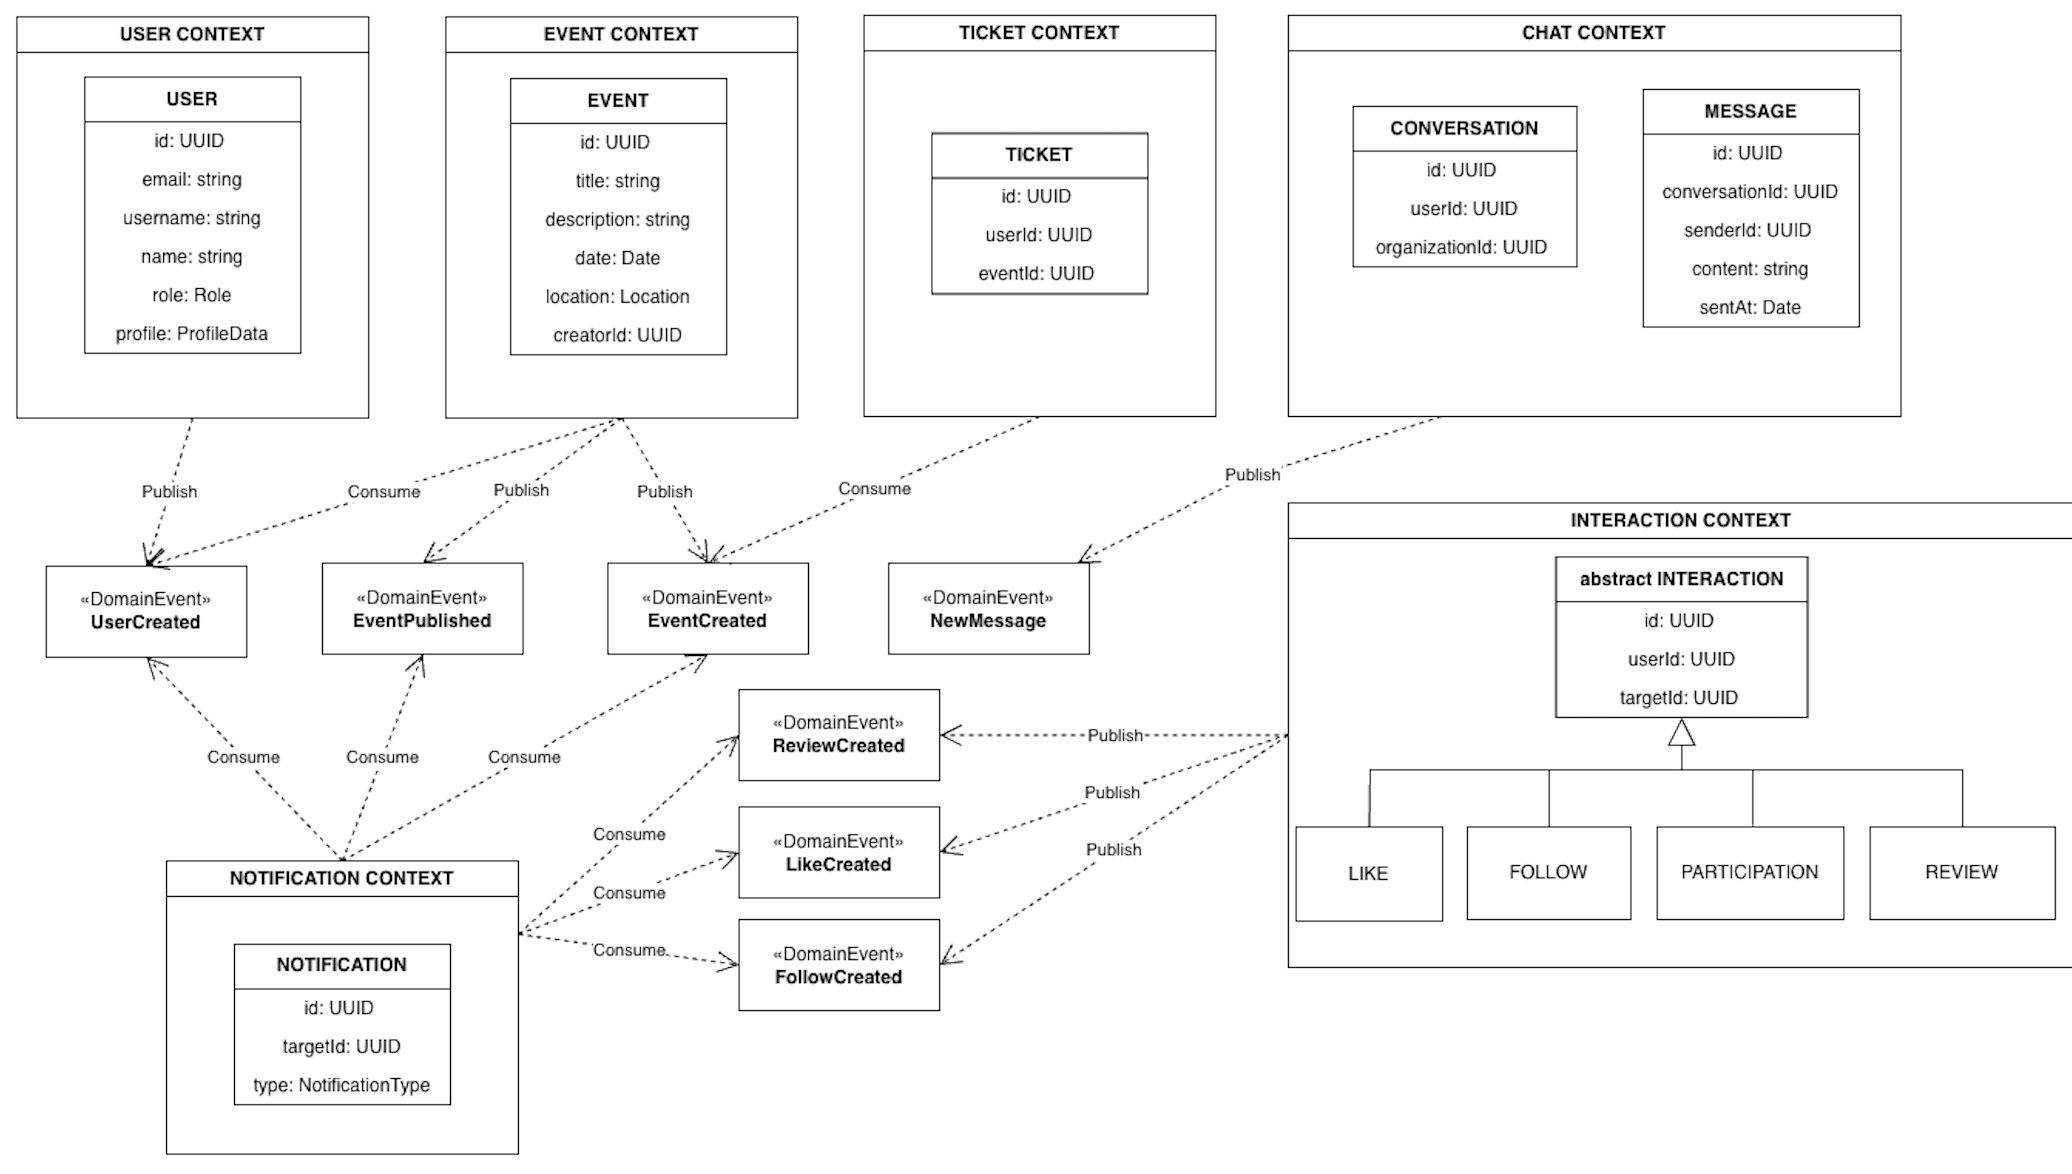
\includegraphics[width=\textwidth]{../public/core-entities.png}
  \caption{Core entities and bounded context diagram}
  \label{fig:core-entities}
\end{figure}

The diagram shows a simplification of the design, not every aspect of the model is represented in details.

The diagram highlights the separation between bounded contexts and the absence of direct structural dependencies across services.

Cross-service relationships are expressed through other entities identifier and domain events rather than object references or shared persistence.

\paragraph{User}
Represents a platform account.
A User can assume one of two roles:
\begin{itemize}
  \item Member
  \item Organization
\end{itemize}
Attributes include identifier, authentication-related data (account), profile information and events preferences.

\paragraph{Event}
Represents an activity created by an Organization.

Its attributes include identifier, title, description and all informations about event (e.g. date, time, location).

\paragraph{Ticket}
Represents a User's receipt of payment to participate in a Event.

It has its own lifecycle (creation, validation or invalidation) and is modeled independently from Event to avoid coupling financial logic with event management logic.

\paragraph{Interaction}

Abstract concept representing user actions.

In particular:
\begin{itemize}
  \item Like (User $\to$ Event)
  \item Follow (User $\to$ User)
  \item Review (User $\to$ Event)
  \item Participation (User $\to$ Event)
\end{itemize}

Interactions are separated from Event and User entities to enable event-driven propagation of user activities, allowing them to evolve independently from core domain entities.

\paragraph{Conversation}

Represents a communication channel between two Users. This entity stores information about the participants involved in the chat and metadata related to the conversation.

Messages are modeled as a separate entity rather than being embedded directly within the Conversation entity. This separation prevents unbounded data growth inside the conversation and allows message data to be managed independently.

Moreover, this design improves efficiency when retrieving the list of conversations. When a user requests the list of active conversations, the system only needs to access conversation metadata without loading all the associated messages. Message data is retrieved only when a specific conversation is opened.

\paragraph{Notification}

Represents a system-generated alert that must be sent to specific user.

Examples:
\begin{itemize}
  \item new follower
  \item new event published from followed organization
  \item new message/like/review received
\end{itemize}

Notifications are derived entities: they originate from domain events generated by other services.

\subsubsection{Domain Events}

In addition to static entities, the system models domain events to improve communication between services.

Examples include:
\begin{itemize}
  \item \texttt{UserCreated}
  \item \texttt{EventCreated}
  \item \texttt{EventPublished}
  \item \texttt{TicketPurchased}
  \item \texttt{LikeAdded}
  \item \texttt{NewMessage}
\end{itemize}

Domain events enable asynchronous integration between bounded contexts and allow the system to maintain eventual consistency.

\subsection{Interaction}

Communication between the different components of the system follows two interaction patterns: synchronous request--response and asynchronous event-based communication.

The choice of combining these two approaches allows the system to support direct user interactions while maintaining loose coupling and independent evolution of backend services.

\begin{itemize}
  \item \textbf{Synchronous interactions between frontend and backend services}:
  Synchronous communication is primarily used for interactions initiated by users through the frontend. In this pattern, a client sends a request to a service and waits for a response before continuing the execution.

  This approach is suitable for operations that require an immediate result, such as authentication, event browsing, or ticket purchasing. The response returned by the service confirms the successful execution of the operation or reports possible errors.
  Using synchronous interactions for user-driven operations simplifies the control flow and ensures that the user receives immediate feedback from the system.

  \item \textbf{Asynchronous event-driven communication}:
  Communication between backend services is primarily handled through asynchronous event-driven interactions. In this model, when a service completes an operation that may affect other parts of the system, it emits a domain event describing the change that occurred.
  Other services can subscribe to the events they are interested in and react accordingly. For example, the creation of an interaction or the publication of an event may trigger the generation of notifications or updates in other subsystems.
\end{itemize}

\paragraph{Consistency and coordination.}

Each service guarantees consistency within its own boundaries by executing state-changing operations within local transactions. After a transaction completes, the service may emit one or more domain events describing the resulting state change.

Other services process these events asynchronously, updating their own state or triggering additional operations. This approach avoids the need for distributed transactions across services and allows the system to maintain overall coherence through eventual consistency.

\subsection{Behaviour}

All of the services in the system follow a common behavioral structure when handling both user requests and inter-service communication.
The goal of this design is to maintain strong consistency within each service while enabling coordination between services in a distributed environment.

Three main behavioral patterns can be identified: request-driven operations, event-driven processing and real-time notification propagation.

\subsubsection{Request-Driven Operations}

User actions are processed through a request-driven workflow. A request is received by the API interface of the corresponding service and forwarded to the layer responsible for executing the domain logic.

To guarantee consistency, operations that modify the system state are executed within a local transactional boundary.

To guarantee reliability, it's adopted the \textbf{Outbox Pattern}. Instead of publishing events directly after the state update, domain events are first stored in a dedicated outbox structure within the same transaction as the database update. This ensures that the state change and the corresponding domain event recording occur atomically.
Once the transaction successfully completes, the events stored in the outbox can be asynchronously delivered to the message broker.

The typical workflow can therefore be summarized as follows:
\begin{enumerate}
  \item A client request is received through the service API.
  \item The request is validated and processed (optionally, also making synchronous request to other services) by the service logic.
  \item A local transaction updates the service state and if necessary records in the outbox the domain events describing the change.
  \item After the transaction completes, the events are asynchronously published.
\end{enumerate}

This pattern guarantees internal consistency within the service while enabling reliable propagation of domain events to the rest of the system.

\begin{figure}[H]
  \centering
  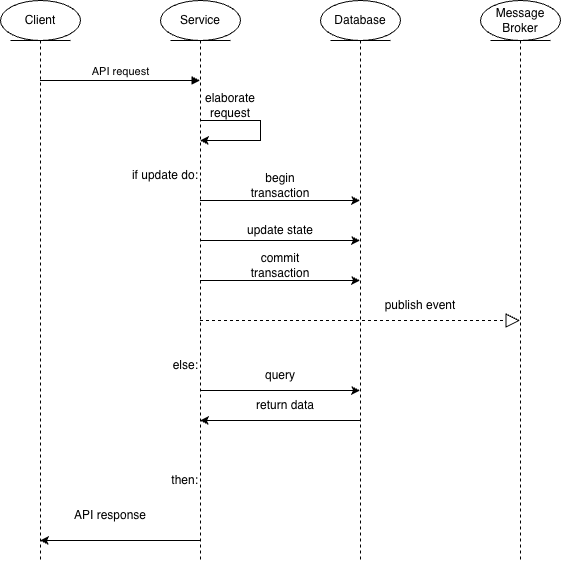
\includegraphics[width=0.7\textwidth]{../public/design/behavior-request-driven.png}
  \caption{Request-driven behavior}
  \label{fig:behavior-request-driven}
\end{figure}

\subsubsection{Event-Driven Processing}

Services also react to domain events generated by other services.
When an event is received, the service processes it through its domain logic and may update its internal state or trigger additional events.

This approach enables coordination between bounded contexts without requiring direct dependencies between services.

The typical flow for this interaction is:
\begin{enumerate}
  \item A domain event is received.
  \item The service processes the event through its domain logic.
  \item If required, a local transaction updates the service state.
  \item Additional domain events may be generated.
\end{enumerate}

This event-driven approach allows services to collaborate asynchronously while preserving loose coupling and independent evolution.

\begin{figure}[H]
  \centering
  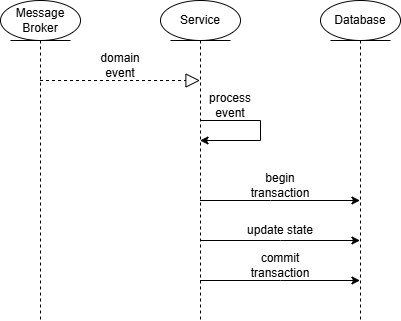
\includegraphics[width=0.7\textwidth]{../public/design/behavior-event-driven.png}
  \caption{Event-driven behavior}
  \label{fig:behavior-event-driven}
\end{figure}

\subsubsection{Real-Time Notification Propagation}

A specific behavior is implemented for real-time user notifications.
Some domain events represent user actions that must be sent to other users, such as a message or a new interaction. These events trigger the creation of notification entities.

The notification subsystem processes the relevant events, stores the corresponding notification and propagates it to connected clients through a real-time communication channel.

The workflow is the following:
\begin{enumerate}
  \item A domain event is generated by a service.
  \item The notification subsystem consumes the event.
  \item A notification entity is created and stored.
  \item The notification is delivered to relevant connected clients in real-time.
\end{enumerate}

This mechanism allows the system to react promptly to user-relevant events while maintaining a decoupled architecture.

\begin{figure}[H]
  \centering
  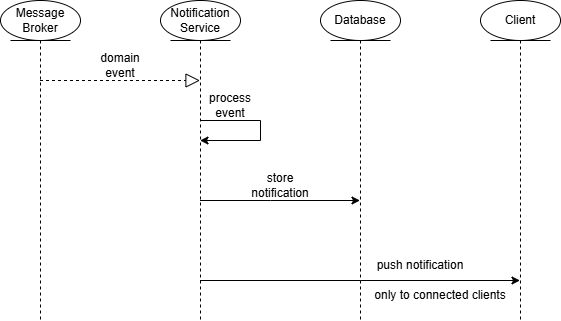
\includegraphics[width=\textwidth]{../public/design/behavior-real-time.png}
  \caption{Real-time notification propagation behavior}
  \label{fig:behavior-real-time}
\end{figure}

\subsection{Architecture}

\subsubsection{Architectural Style}

The system is designed according to a \textbf{microservices architecture}. The application is decomposed into a set of small, independently deployable services, each responsible for a specific bounded context: user, event, interaction, chat, ticketing and notification.

Each microservice encapsulates its own domain logic and adopts the \textbf{database-per-service} pattern.

When shared information is required (e.g., basic user data such as \texttt{id}, \texttt{name} and \texttt{avatar} needed by the \texttt{chat} or \texttt{interaction} services), it is propagated via \textbf{domain events} rather than retrieved through synchronous queries. This intentional data duplication reduces communication overhead and keeps services decoupled.

Moreover, this design avoids the bottleneck that would arise from sharing a single database across multiple services and guarantees strong data ownership by preventing services from directly accessing another service's data store.
\newpage
\noindent\textbf{Inter-service communication}

Two complementary communication styles are adopted:

\begin{itemize}
  \item \textbf{Synchronous (HTTP REST)}: used when fulfilling a request requires invoking an operation or retrieving data from another service, or to propagate state changes immediately to dependent services. For example, when an event is created, the \texttt{event} service notifies \texttt{ticketing} via its internal API so that ticket-related operations can proceed right away.

  \item \textbf{Asynchronous}: used to propagate state changes across service boundaries without creating runtime dependencies between them and to push real-time updates to connected clients. Three mechanisms are in place:
    \begin{itemize}
      \item \textbf{Domain events (RabbitMQ)}: services publish events to the message broker; subscribers consume them independently. For example, when an event is published, the \texttt{event} service emits an \texttt{EventPublished} domain event consumed by the \texttt{notification}, \texttt{ticketing} and \texttt{interaction} services.
      \item \textbf{WebSocket (Socket.IO)}: used by the \texttt{notification} service to maintain persistent connections with clients, enabling server-side push of real-time updates without polling. For example, when \texttt{notification} receives an \texttt{EventPublished} domain event, it delivers an update to the relevant connected clients. In this case, users following the organization that published the event.
      \item \textbf{Webhooks}: used for third-party integrations that push notifications into the system, for example payment provider (Stripe) callbacks delivered to the \texttt{ticketing} service. The receiving service processes the incoming HTTP call asynchronously without blocking any client-facing request.
    \end{itemize}
\end{itemize}

\noindent\textbf{API gateway}

All external traffic flows through an API gateway implemented with \textbf{Traefik}, which acts as a single entry point and keeps the internal service topology invisible to clients.

\medskip
\noindent\textbf{Motivation for the architectural choice}

\begin{itemize}
  \item \textbf{Service independence}: each service can be developed, tested and deployed independently.
  \item \textbf{Scalability}: services can scale horizontally according to their specific load.
  \item \textbf{Loose coupling}: the combination of database-per-service and event-driven communication minimises direct dependencies, improving maintainability.
  \item \textbf{Data isolation}: each service's database schema evolves independently, preventing unintended cross-service coupling.
  \item \textbf{Resilience and fault isolation}: failures are contained within individual services; asynchronous communication through the message broker allows a service to be temporarily unavailable without blocking the rest of the system.
\end{itemize}

\subsubsection{Infrastructure}

\begin{figure}[H]
  \centering
  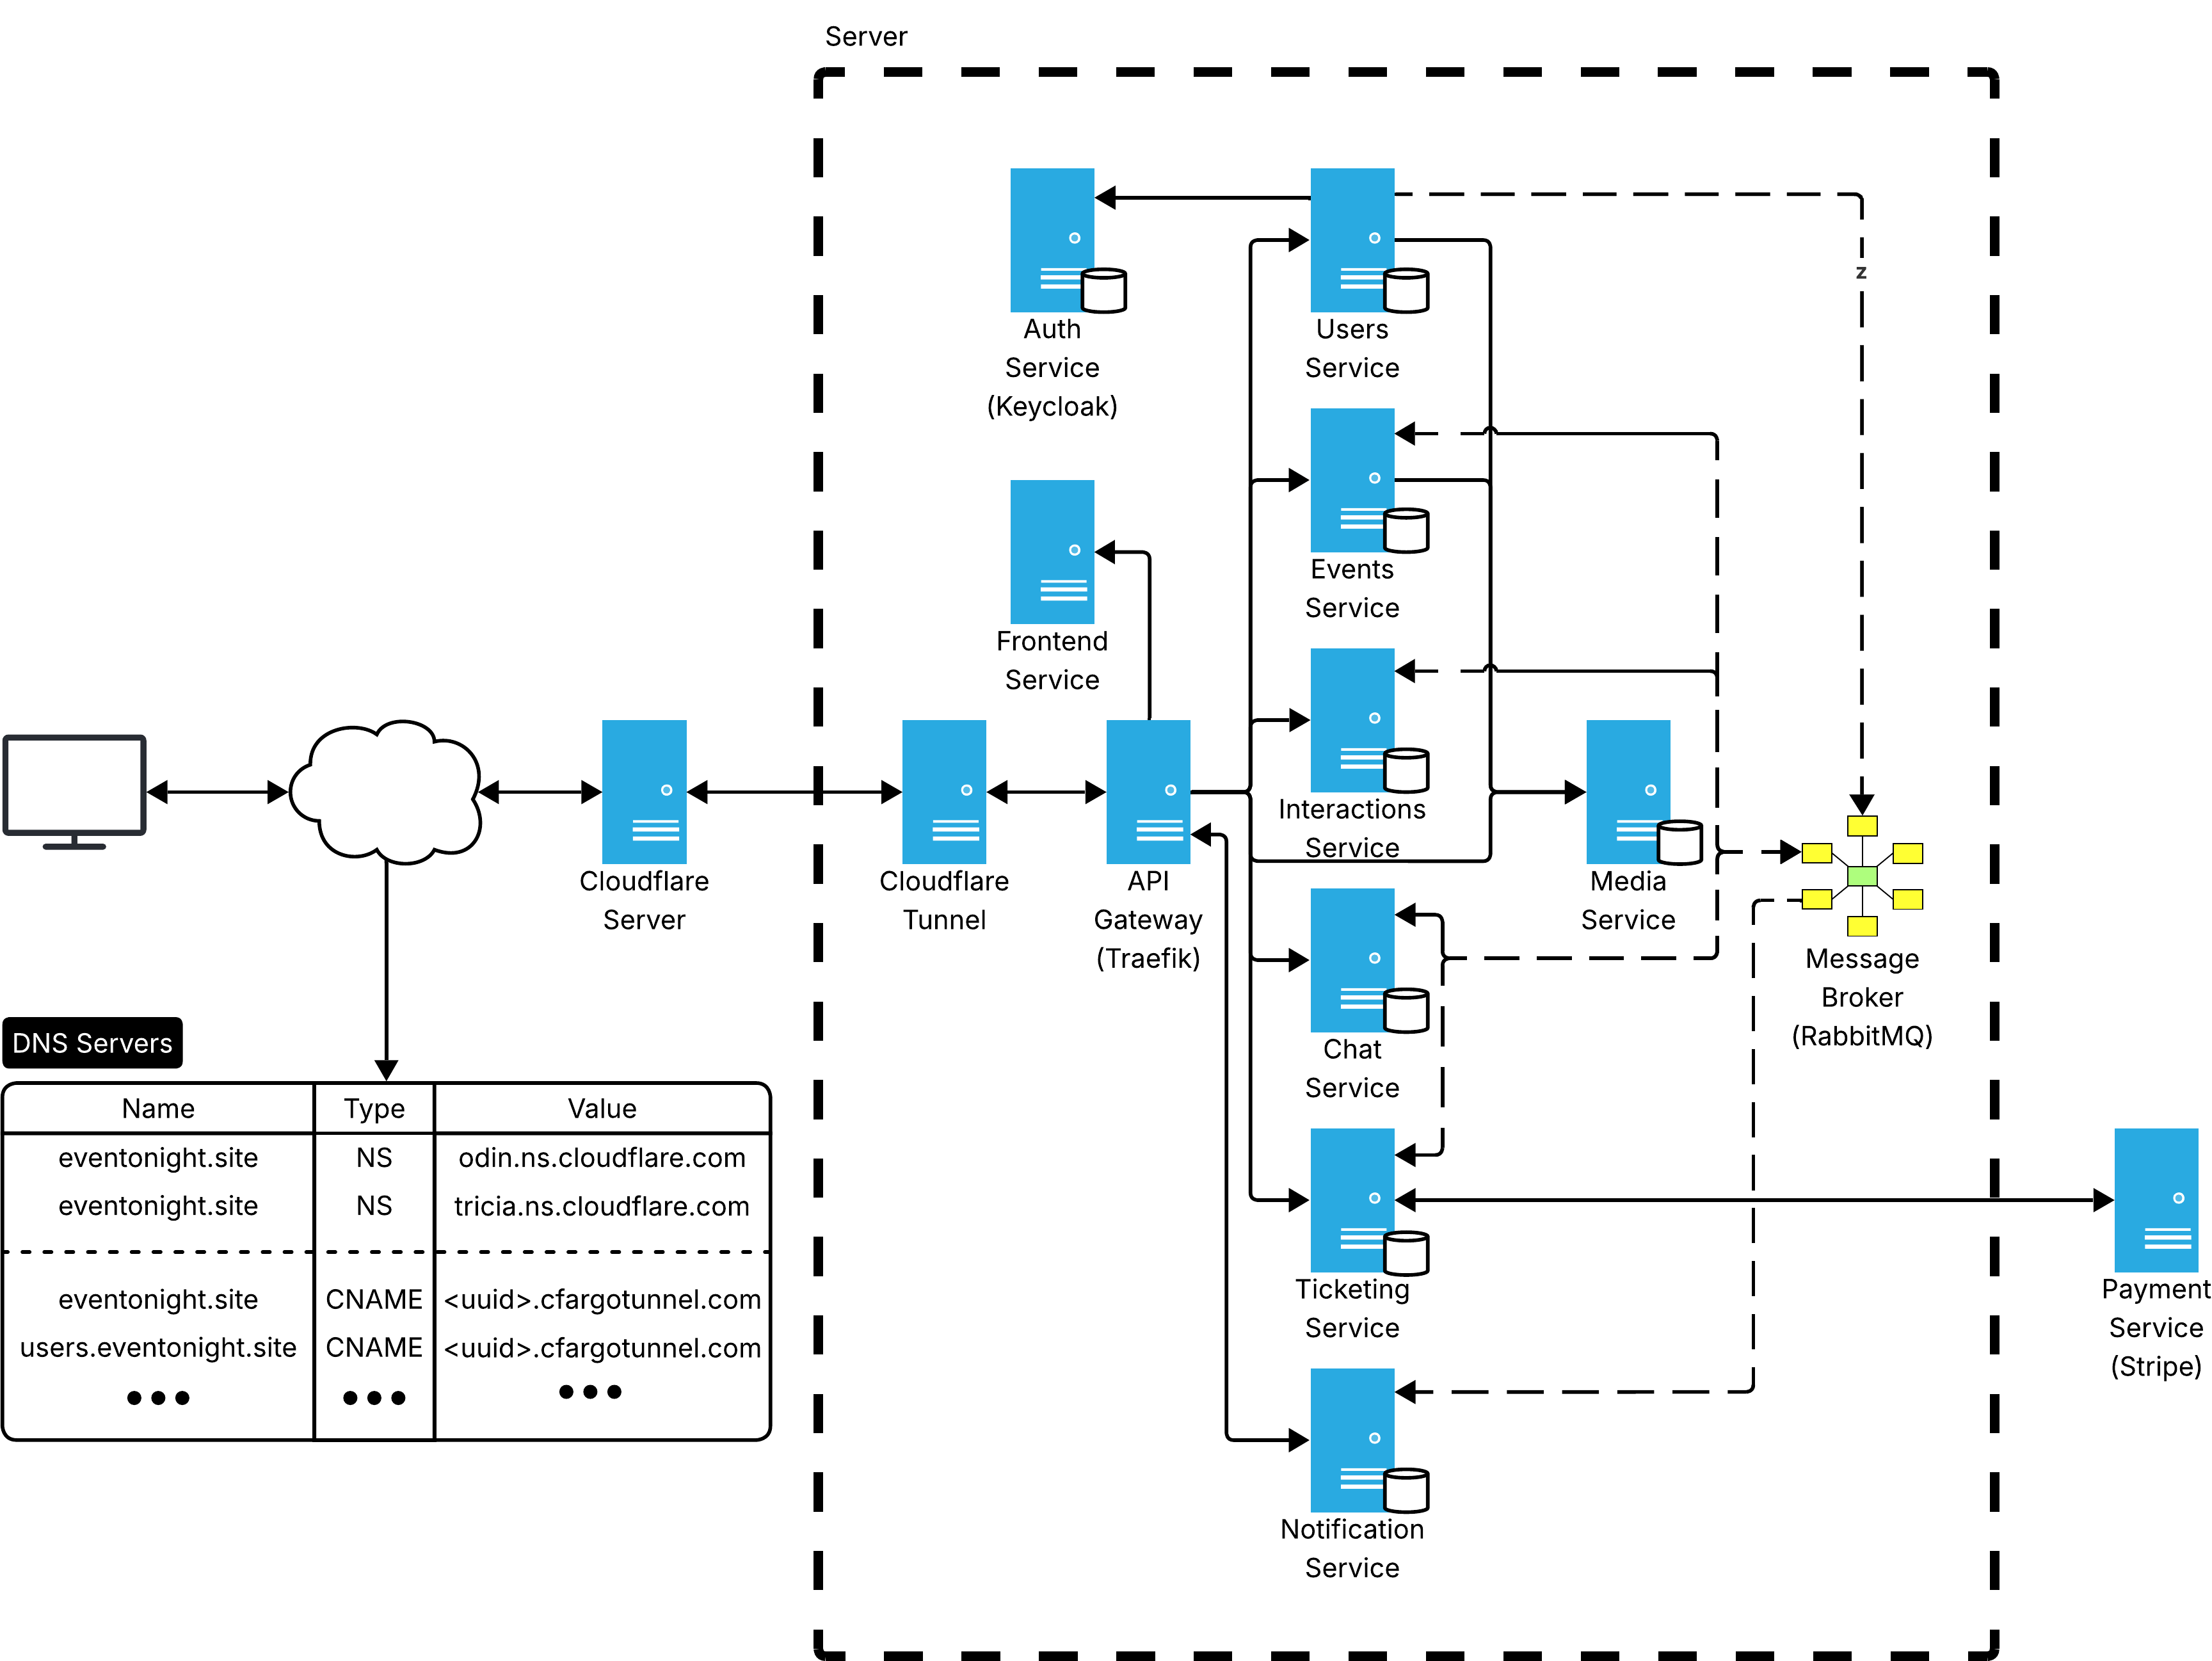
\includegraphics[width=\textwidth]{../public/design/Infrastructure.png}
  \caption{Infrastructure diagram}
  \label{fig:infrastructure}
\end{figure}
\newpage
\noindent\textbf{Components}

All infrastructural components are listed in the table below.

\begin{table}[H]
  \centering
  \begin{tabular}{p{3.2cm}p{3.2cm}p{7cm}}
    \toprule
    \textbf{Component} & \textbf{Technology} & \textbf{Description} \\
    \midrule
    DNS / TLS & Cloudflare & Authoritative DNS and TLS termination \\
    Tunnel daemon & cloudflared & Maintains an outbound encrypted tunnel to Cloudflare; no inbound ports required on the cluster \\
    API gateway / Reverse proxy & Traefik v3 & Single entry point for all external HTTP/WebSocket traffic; handles routing, load balancing, rate limiting, retries, circuit breaking and request timeouts; discovers services via Docker label-based configuration \\
    Backend services & Scala 3 + Cask & \texttt{user}, \texttt{event} \\
    Backend services & NestJS (Node.js) & \texttt{chat}, \texttt{interaction}, \texttt{ticketing} \\
    Backend services & Express (Node.js) & \texttt{media}, \texttt{notification} \\
    Frontend & Vue 3 + Vite & Single-page application served as static assets \\
    Identity provider & Keycloak & User authentication and JWT issuance \\
    Message broker & RabbitMQ & Asynchronous event delivery via a topic exchange \\
    Document databases & MongoDB & One dedicated instance per service \\
    Relational database & PostgreSQL & Backing store for Keycloak \\
    Object storage & MinIO & Binary file and image storage for the \texttt{media} service \\
    Payment provider & Stripe \textit{(external)} & Third-party payment processing \\
    Seed service & Node.js & Populates databases with initial data on first deployment \\
    \bottomrule
  \end{tabular}
  \caption{Infrastructure components}
  \label{tab:infrastructure}
\end{table}

\noindent\textbf{Network distribution}

With the exception of Stripe, all components run inside a single host using \textbf{Docker Compose}. No service port is exposed to the public internet, the only inbound path is through the Cloudflare tunnel.

Two categories of Docker bridge networks are used:

\begin{itemize}
  \item \textbf{\texttt{eventonight-network}}: shared by all application services, Traefik, RabbitMQ and Keycloak. Used for inter-service communication and Traefik routing.
  \item \textbf{\texttt{<service>-network}}: one private network per service, shared exclusively between the service, its database instance and any auxiliary containers (e.g. provisioning scripts that perform initial setup, as in the case of Keycloak). This enforces database isolation, no other service can reach another service's database.
\end{itemize}

\noindent\textbf{Service discovery}

External clients resolve subdomains through Cloudflare's authoritative DNS. Each subdomain is a CNAME record pointing to \texttt{<uuid>.cfargotunnel.com}, which resolves to a Cloudflare edge IP. Traffic enters the cluster through the \texttt{cloudflared} tunnel and is handed off to Traefik.

Inside the host, discovery is handled by Docker Compose:

\begin{itemize}
  \item \textbf{Internal DNS}: Compose registers each service by name in the internal DNS (e.g., \texttt{http://users:9000}, \texttt{amqp://rabbitmq:5672}). No manual registration is required.
  \item \textbf{Traefik routing}: Traefik watches the Docker API for label changes and rebuilds its routing table automatically when services are started or stopped.
\end{itemize}

\subsubsection{Data Flow}

\noindent\textbf{Synchronous request flow (HTTP REST)}

\begin{verbatim}
Browser → Cloudflare (DNS + TLS) → cloudflared
        → Traefik → Service → Database → response
\end{verbatim}

The browser sends an HTTPS request to a subdomain (e.g., \texttt{events.eventonight.site}). Cloudflare resolves the DNS and terminates TLS, then injects the request into the persistent encrypted tunnel (QUIC) maintained by \texttt{cloudflared} on the cluster. Traefik receives it, matches the \texttt{Host} header against its routing rules and forwards the request to the target service. The service handles the request, queries its own database instance and returns the response through the same chain.

\medskip
\noindent\textbf{Asynchronous event flow (AMQP)}

\begin{verbatim}
Service → Exchange (eventonight) → Queue (per-service) → Consumer service
\end{verbatim}

\begin{figure}[H]
  \centering
  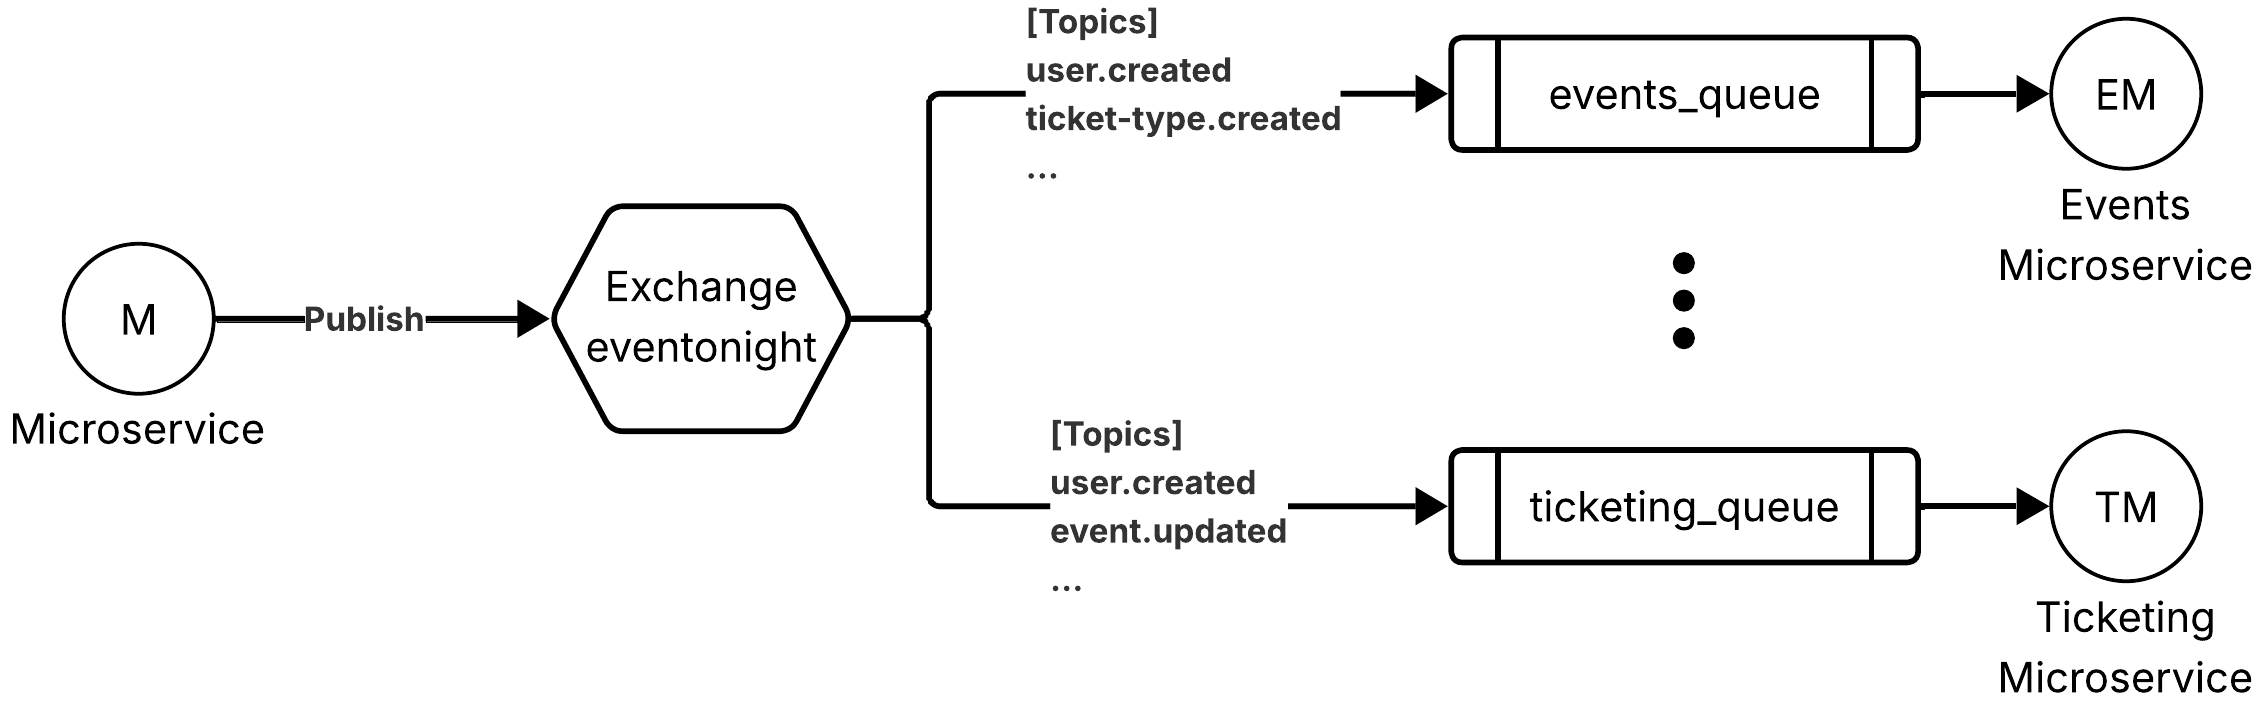
\includegraphics[width=\textwidth]{../public/design/Broker.png}
  \caption{Message broker topology}
  \label{fig:broker}
\end{figure}

RabbitMQ uses a single \textbf{topic exchange} named \texttt{eventonight}. Each consuming service has a dedicated queue bound to the exchange with a set of topic subscriptions (e.g., \texttt{ticketing\_queue} binds to \texttt{user.created}, \texttt{event.updated} and many others). When a service publishes a domain event with a routing key, the exchange fans it out to every queue whose binding pattern matches, without the publisher knowing who the consumers are.

\newpage
\noindent\textbf{Real-time push (WebSocket)}

\begin{verbatim}
notification service → Socket.IO → Browser
\end{verbatim}

The \texttt{notification} service consumes events from its queue and pushes real-time updates to the relevant connected clients over WebSocket (Socket.IO).

\medskip
\noindent\textbf{Webhook flow (Stripe $\to$ ticketing)}

\begin{verbatim}
Stripe → Cloudflare → cloudflared → Traefik
       → ticketing (acknowledged immediately, processed asynchronously)
\end{verbatim}

Stripe delivers payment event callbacks via HTTP POST to the \texttt{ticketing} service. The service responds immediately with \texttt{200 OK} and processes the event asynchronously, without blocking any client-facing operation.

\subsubsection{Web API}

All application services expose a \textbf{REST API}, accessible externally via Traefik at \texttt{<service>.even\allowbreak tonight.site}. Every protected endpoint requires a \textbf{JWT Bearer token} in the \texttt{Authorization} header, issued by Keycloak and validated independently by each service using Keycloak's public key, no centralised auth gateway is needed.
The \texttt{notification} service additionally exposes a \textbf{WebSocket endpoint}.

\subsubsection{Scalability and High Availability}

The current deployment runs all components on a \textbf{single host} using Docker Compose. Each service runs as a single container instance, which provides basic availability but represents a single point of failure at the host level.
The architecture below is designed to transition to \textbf{high availability} by adopting \textbf{Docker Swarm}.

\begin{figure}[H]
  \centering
  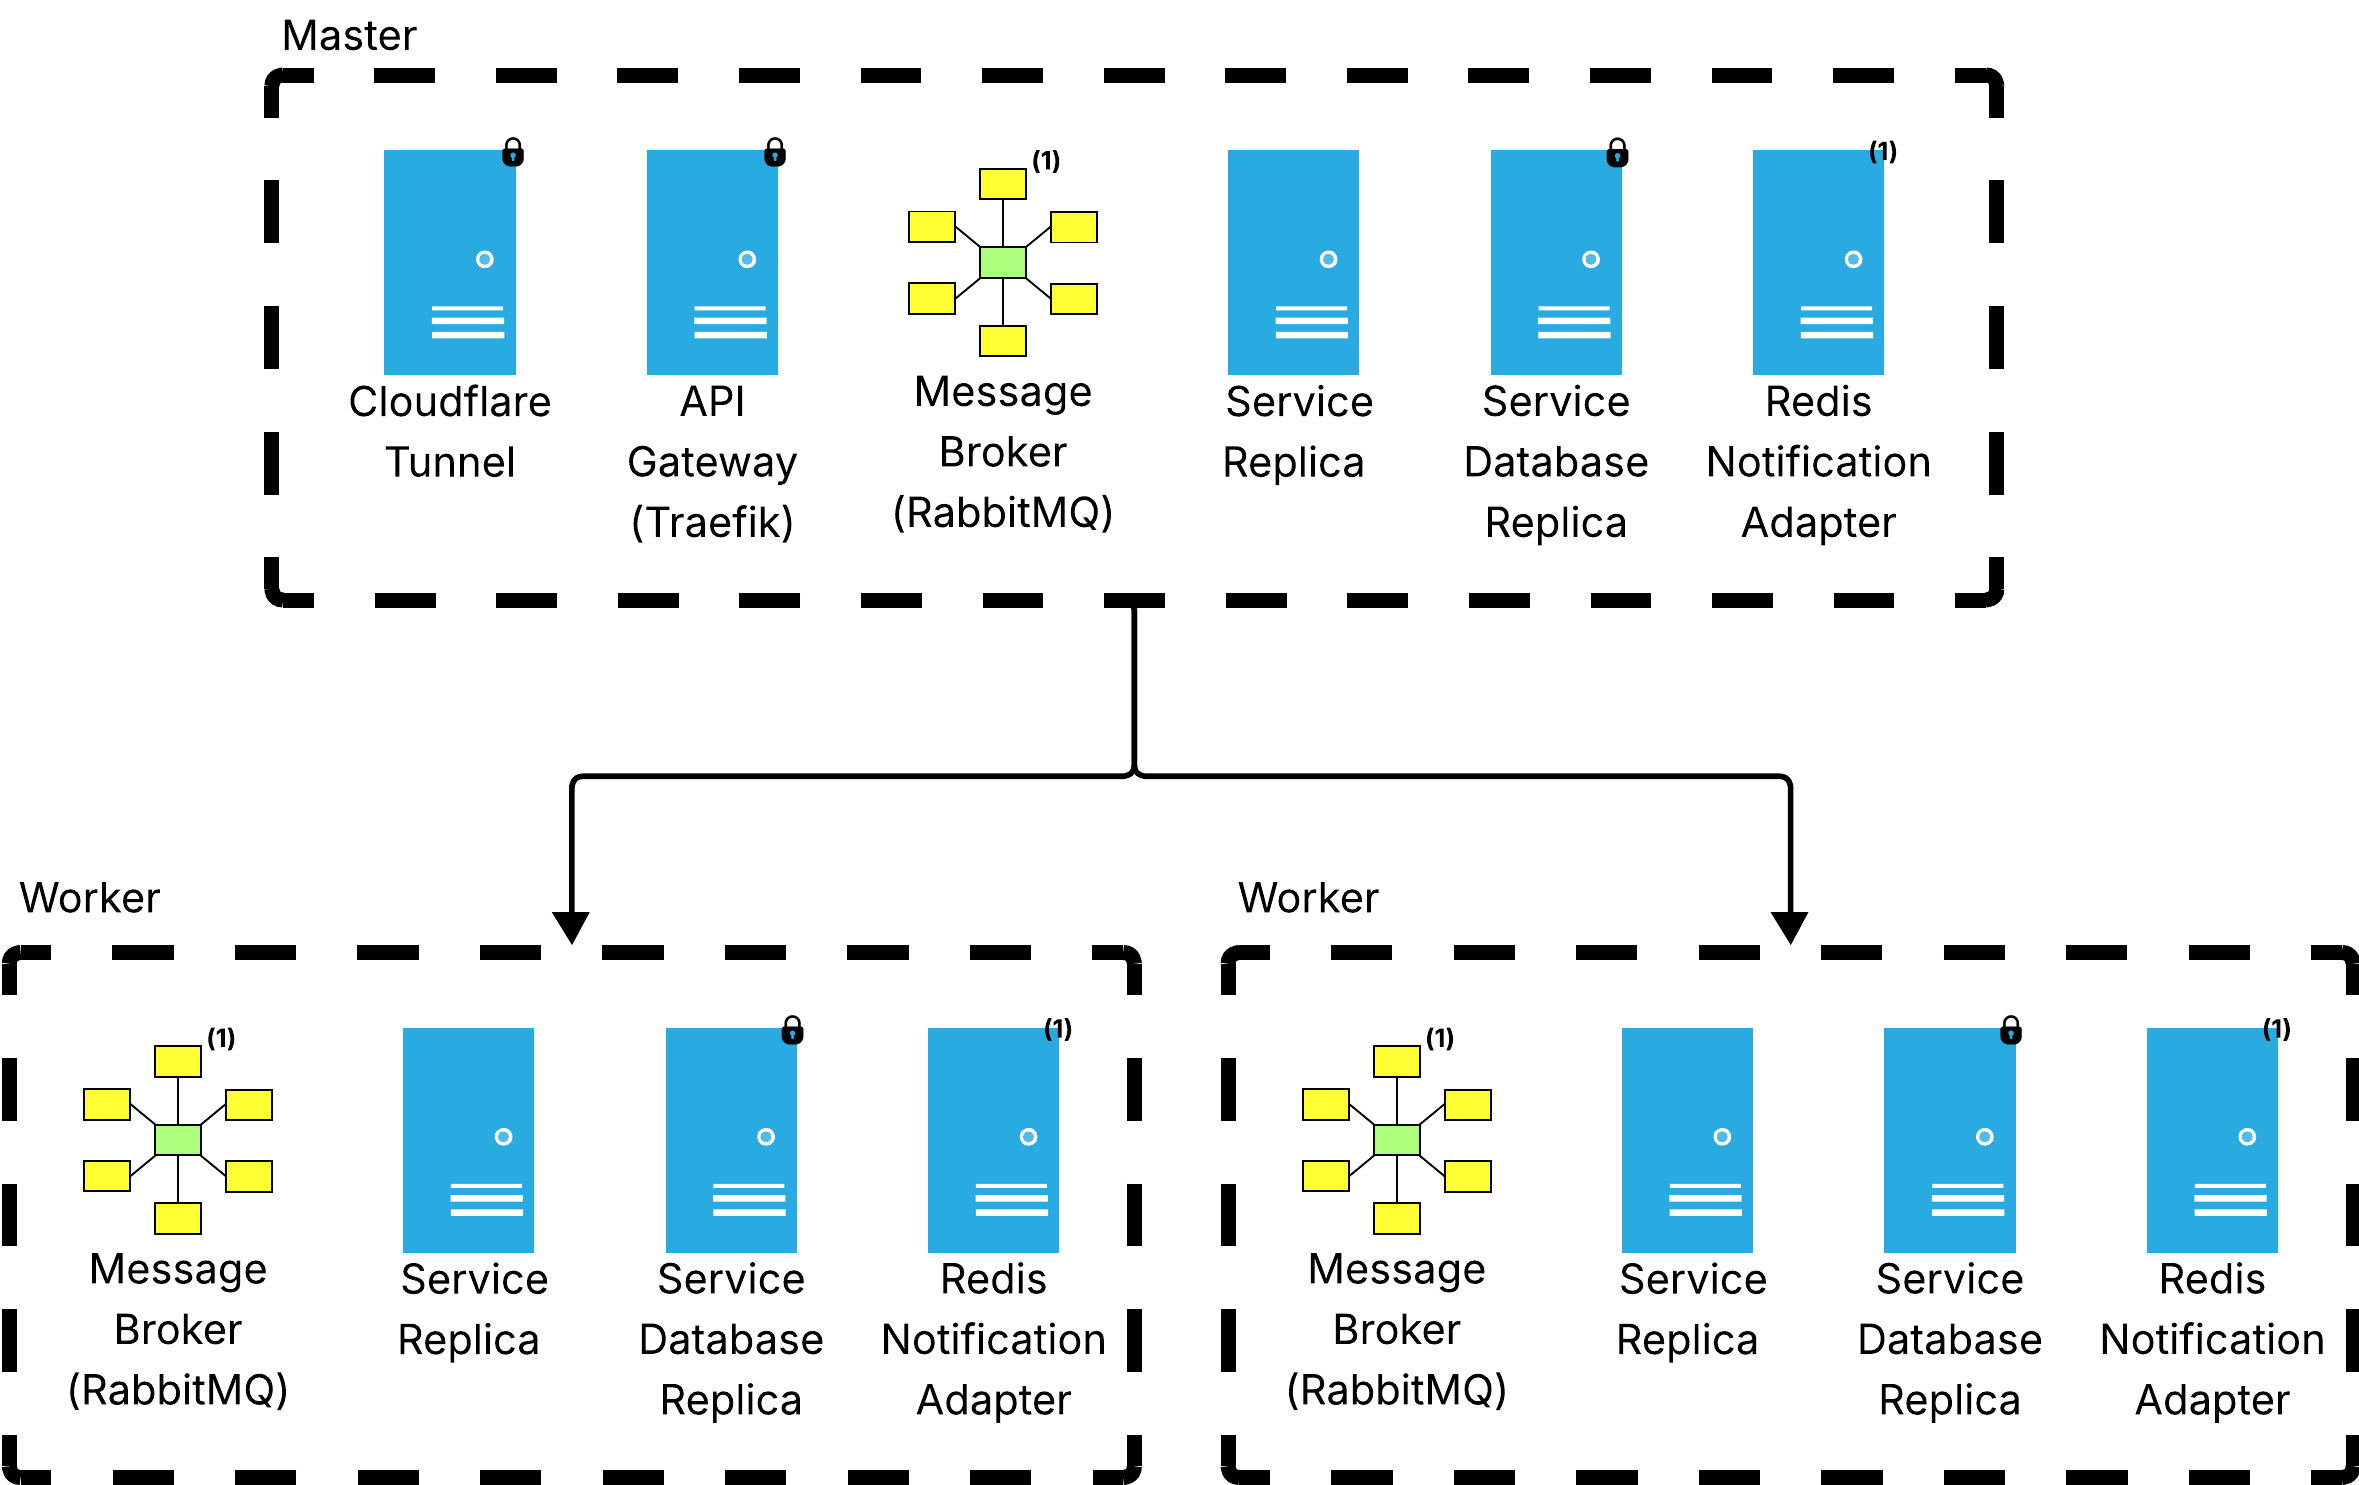
\includegraphics[width=0.9\textwidth]{../public/design/Swarm.png}
  \caption{Docker Swarm deployment topology}
  \label{fig:swarm}
\end{figure}

Even on a single node, Swarm already provides a first step toward HA through \textbf{rolling updates}, services can be updated replica by replica with zero downtime, unlike a plain Compose deployment where an update implies a brief interruption. Moving to a multi-node cluster then enables true HA by distributing replicas across machines, so that the failure of a node does not take down the service.

However, adding nodes and replicas is a necessary but not sufficient condition for HA, it also requires deliberate design choices at the infrastructure level and at the application level to preserve correctness: stateful services require dedicated replication strategies and deploying multiple replicas of a service introduces competing consumer scenarios on the broker that must be explicitly handled.

\medskip
\noindent\textbf{Cluster topology}

For true HA, the Swarm should have at least \textbf{three manager nodes}. Swarm managers use the Raft consensus protocol to maintain cluster state and an odd number of managers is required to form a quorum and tolerate node failures (three managers tolerate one failure). Each manager node should run its own Traefik and \texttt{cloudflared} instance, so Cloudflare load-balances incoming traffic across all managers automatically.

\medskip
\noindent\textbf{Service placement}

Stateless application services can be freely distributed across nodes. Stateful services (RabbitMQ and databases) require \textbf{placement constraints} to be distributed and binded on different machines. Manager nodes should be set to \textbf{drain} availability so the Swarm scheduler assigns no application workloads to them, keeping them dedicated exclusively to cluster management and incoming traffic.

\medskip
\noindent\textbf{Message broker with multiple consumers}

Scaling application services to multiple replicas introduces a non-trivial consideration for broker consumption. The current setup uses a \textbf{single active consumer} per queue: only one replica consumes from a given queue at a time, guaranteeing FIFO message processing. This is sufficient for HA because if the active consumer fails, another replica takes over, but it does not improve throughput.

To scale throughput beyond a single consumer, more refined strategies can be explored:

\begin{itemize}
  \item \textbf{Consistent hash exchange}: a RabbitMQ plugin that replaces the standard topic exchange with a hashing layer. Using that, messages are routed to one of N queues based on a hash of the routing key, allowing N consumers to process in parallel while preserving per-key ordering.
  \item \textbf{Streams / Super Streams}: RabbitMQ Streams provide a persistent, replayable log. Super Streams partition a logical stream across multiple physical streams, each consumed by a dedicated replica, combining throughput scaling with ordering guarantees per partition.
  \item \textbf{Sequence fields}: adding a monotonically increasing \texttt{version} or \texttt{seq} field per entity allows consumers to detect and discard out-of-order messages regardless of the consumption strategy adopted.
\end{itemize}

\noindent\textbf{What changes with Swarm:}

\begin{itemize}
  \item \textbf{\texttt{cloudflared} and Traefik} scale with the number of manager nodes, one instance per manager. Traefik natively supports Swarm mode via the Docker API.
  \item \textbf{Stateless application services} can be scaled to multiple replicas and distributed freely across nodes.
  \item \textbf{Stateful services} require dedicated HA strategies: MongoDB moves to a \textbf{replica set} (primary + secondaries) and RabbitMQ to a \textbf{quorum queue cluster}, both require an odd number of members (e.g. 3, 5) to guarantee quorum and avoid split-brain, ensuring data redundancy and automatic failover. Each stateful instance must be pinned to a distinct node (at most one replica per node) so that a single node failure does not take down multiple members of the same cluster. Replicated data stores also improve \textbf{fault tolerance}, the system continues to operate and preserves data integrity even if individual nodes are lost.
  \item \textbf{WebSocket sticky sessions}: when \texttt{notification} runs as multiple replicas, Traefik must be configured with a sticky cookie to ensure Socket.IO handshake and subsequent frames are consistently routed to the same replica. However, sticky sessions alone are not sufficient: to broadcast events to all connected clients regardless of which replica they are connected to, a \textbf{Redis adapter} for Socket.IO is required to propagate messages across all instances.
\end{itemize}

\subsection{Corner Cases}

The system is designed to be \textbf{highly available} and \textbf{eventual consistent}. Each service operates independently and failures are isolated: when a component goes down, only the functionality directly depending on it is affected, while the rest of the system continues to operate.

\paragraph{Fault detection.}
Each service exposes a \texttt{/health} endpoint and declares a \texttt{healthcheck} in Docker Compose. This allow Docker to automatically restarts or reschedules tasks that become unhealthy, making fault detection active. To further improve observability, a dedicated monitoring service could be introduced.

\paragraph{Startup ordering and reconnection.}
In a Compose deployment, dependent services use \texttt{depends\_on} with \texttt{condition: service\_healthy} to enforce startup ordering. In a Swarm deployment this mechanism is not available: each service must instead be resilient to the temporary unavailability of its dependencies and implement reconnection logic autonomously. Note that reconnection logic is necessary regardless of the deployment model, as dependencies may also fail and recover during normal operation. All reconnection attempts, to MongoDB, RabbitMQ and other services, use an exponential backoff strategy.

\paragraph{Error signalling.}
Every API endpoint returns standard HTTP status codes to communicate failures to clients: \texttt{400} for validation errors, \texttt{401} for missing or invalid tokens, \texttt{403} for authorisation failures, \texttt{404} for resources not found, \texttt{409} for conflicts, \texttt{500} for unexpected server errors and so on. With a monitoring service in place, an alerting mechanism can be added to proactively notify on service failures.

\paragraph{Component failure and recovery.}
In a Compose deployment, all containers run with \texttt{restart: unless-stopped}, so Docker automatically restarts any crashed container. Docker itself is configured to start on host boot, meaning that even a full machine reboot brings the entire system back up without manual intervention. In a Swarm deployment, the restart policy is managed by the Swarm scheduler, which restarts failed tasks and, if a node goes down, reschedules its tasks onto healthy nodes automatically. In both cases, full recovery is achieved because services are resilient to dependency failures and re-establish connections autonomously.

\paragraph{Database failure.}
If a MongoDB instance goes down, its owning service remains partially operational: requests that do not require the database can still be served. The service reconnects automatically when the database comes back up. In a Swarm deployment with a replica set, a single node failure triggers an automatic primary election and the service reconnects to the new primary, avoiding a full outage. In both cases, multi-document operations are executed within MongoDB transactions, so a crash mid-operation leaves no inconsistent state, the transaction is simply rolled back.

\paragraph{Service failure.}
If a service crashes, Docker restarts it automatically. Since all writes are transactional, there is no risk of partial state being committed. However when a service crashes after initiating an outbound HTTP call to an external system (e.g. creating a Stripe checkout session or a Keycloak user) but before completing its local operations, an inconsistency may arise: the side effect on the external system has already occurred but the local state does not reflect it. In these cases specific strategy must be applied for each integration to handle it correctly.

\paragraph{RabbitMQ failure.}
All queues are declared as durable with persistent messages, so any message received by RabbitMQ before it goes down is safely stored to disk and delivered to consumers once it restarts. In a Swarm deployment with a quorum queue cluster, a single node failure does not cause an outage, the cluster continues operating as long as a majority of nodes are available and messages are replicated across them. RabbitMQ provides at-least-once delivery semantics; services handle this by designing message handlers to be idempotent. If RabbitMQ is unavailable at the moment a service needs to publish, messages are not lost since each service implements the outbox pattern.

\paragraph{Keycloak failure.}
If Keycloak goes down new logins and token refreshes will fail. However, services validate JWTs locally using Keycloak's public key, so requests carrying a still-valid token continue to be accepted until expiry. Once Keycloak restarts, authentication resumes normally.

\paragraph{Traefik or cloudflared failure.}
In a Compose deployment, external traffic cannot enter the system until Docker restarts the container and access resumes. In a Swarm deployment, both run one instance per manager node, so a single manager failure does not interrupt external traffic, Cloudflare simply routes through the remaining instances.

\paragraph{Ticketing crash during checkout session creation.}
If \texttt{ticketing} crashes after tickets have been reserved and the Stripe session has been created, but before send response to the client, the session will eventually expire and Stripe delivers a \texttt{checkout.session.expired} webhook allowing \texttt{ticketing} to release the reserved tickets. If the crash occurs before the Stripe session is created, no webhook will ever arrive and the tickets remain stuck in \texttt{PENDING}; a background cleanup job on timed-out pending orders would be needed to handle this case.

\paragraph{Ticketing unavailability.}
Webhook callbacks from Stripe cannot be processed. Stripe automatically retries undelivered events for up to three days, so the \texttt{ticketing} service will receive and process them once it recovers, without any data loss.

\paragraph{Dual notification path (sync + async).}
When an event is created, the \texttt{event} service notifies \texttt{ticketing} synchronously via HTTP call to an internal endpoint, without waiting for the asynchronous domain event to arrive. The RabbitMQ message still follows as a fault-tolerance fallback.

\paragraph{User crash during register and password update.}
If \texttt{user} crashes after creating the account in Keycloak but before persisting the user record locally, the user exists in the identity provider but not in the \texttt{user} service. On the next login attempt, Keycloak authenticates the user and issues a valid JWT, but \texttt{user} has no matching record. A recovery strategy can be to detect this condition at login time and create a minimal empty profile automatically, mirroring what registration would have done. For password updates, a crash mid-operation leaves the state consistent but the user may not have been correctly notified of the outcome; a "forgot password" flow provides a user-friendly self-service recovery path in this case.

\paragraph{Consistent backup.}
Because each service owns its own database, there is no single point from which to take a globally consistent snapshot. Backing up each database independently means the captured states may be at slightly different points in time. Full cross-service consistency at backup time is not achievable without a distributed snapshot protocol. One practical mitigation is to temporarily halt writes across all services, snapshot all databases simultaneously, then resume, guaranteeing consistency at the cost of a short downtime.

\newpage
\section{Salient Implementation Details}

Full API documentation has been produced for all services:
\begin{itemize}
  \item \href{https://eventonight.github.io/EvenToNight/openAPI/}{\textbf{OpenAPI specs} (REST)}
  \item \href{https://eventonight.github.io/EvenToNight/asyncAPI/}{\textbf{AsyncAPI specs} (RabbitMQ)}
\end{itemize}

The sections below cover implementation choices not captured by the API specifications.

\subsection{Technological Details}

\paragraph{In-transit data representation.} All REST APIs and RabbitMQ messages use \textbf{JSON} as the serialization format.

\paragraph{Database querying.} All application services use \textbf{MongoDB} as their document store:

\begin{itemize}
  \item \texttt{user} and \texttt{event} (Scala) query MongoDB via the raw Java driver (\texttt{mongodb-driver-sync}).
  \item \texttt{chat}, \texttt{interaction}, \texttt{notification} and \texttt{ticketing} (Typescript) use \textbf{Mongoose} as the ODM, with schema decorators and typed model queries.
\end{itemize}

The \texttt{media} service stores binary files in \textbf{MinIO}, an S3-compatible self-hosted object store. PostgreSQL is only used internally by Keycloak.

\paragraph{Authentication.} Authentication is handled by \textbf{Keycloak}. On login, Keycloak issues a short-lived JWT access token and a longer-lived refresh token. Every protected API endpoint requires an \texttt{Authorization: Bearer <token>} header. Each service validates the JWT independently using Keycloak's RSA public key, the \texttt{user} service exposes a \texttt{/public-keys} endpoint that the other services fetch at startup. No centralised auth gateway is involved in validating requests.

The frontend stores tokens in \texttt{sessionStorage}, automatically refreshes the refresh token before expiry and injects access token into all outgoing requests.

\paragraph{Authorization.} The system uses \textbf{Role-Based Access Control (RBAC)} with two roles: \texttt{member} and \texttt{organization}. Roles are assigned in Keycloak at registration time and embedded in the JWT. Services extract the role from the token and apply authorization logic at the handler level, for example, only an \texttt{organization} can create events and only the owning user can modify their own resources.

\paragraph{RabbitMQ message format.} All domain events published to the \texttt{eventonight} topic exchange share a common envelope:

\begin{lstlisting}[]
{
  "eventType": "event.published",
  "occurredAt": "2025-01-01T12:00:00Z",
  "payload": { ... }
}
\end{lstlisting}
\captionof{lstlisting}{Domain event envelope}
\label{lst:event-envelope}

\paragraph{MongoDB single-node replica set.} MongoDB transactions require a replica set. All services run MongoDB in replica set mode even on a single node, using \texttt{--replSet rs0} and initialising a one-member replica set at startup. This setup unlocks multi-document transaction support and makes the transition to a multi-node replica set in a Swarm deployment straightforward, with no changes required to the application layer.

\paragraph{Stripe webhook authentication.} Stripe signs every webhook payload using a secret. The \texttt{ticketing} service verifies this signature before processing any incoming webhook, ensuring that only legitimate Stripe events are accepted.

\paragraph{Socket.IO: authenticated connections and scaling.} WebSocket connections to the \texttt{notification} service are authenticated: the client sends its JWT and \texttt{userId} during the Socket.IO handshake and the server validates the token before allowing the connection. Socket.IO was chosen over raw WebSocket also because it natively supports a Redis pub/sub adapter, which would allow the \texttt{notification} service to scale horizontally across multiple replicas while still delivering pushes to the correct client regardless of which replica it is connected to.

\paragraph{Key implementation patterns.}
\begin{itemize}
  \item \textbf{Transactional outbox}: each service writes domain events to an outbox collection atomically with the state change (within a MongoDB transaction); a relay process forwards them to RabbitMQ, retrying with exponential backoff until delivery succeeds. This decouples message publishing from the availability of RabbitMQ.

  \item \textbf{Saga pattern}: the ticket purchase flow is implemented as a two-phase saga. Phase 1 reserves inventory and creates an order atomically in MongoDB (TX1). Phase 2 calls Stripe to create a checkout session. If Stripe fails, a compensating transaction releases the reserved tickets and cancels the order. If the service crashes between the two phases, the compensation does not run, tickets remain in \texttt{PENDING} state indefinitely. The correct mitigation would be a scheduled cleanup job that releases orders stuck in \texttt{PENDING} beyond a timeout threshold; this is a known limitation of the current implementation.
\end{itemize}

\begin{figure}[H]
  \centering
  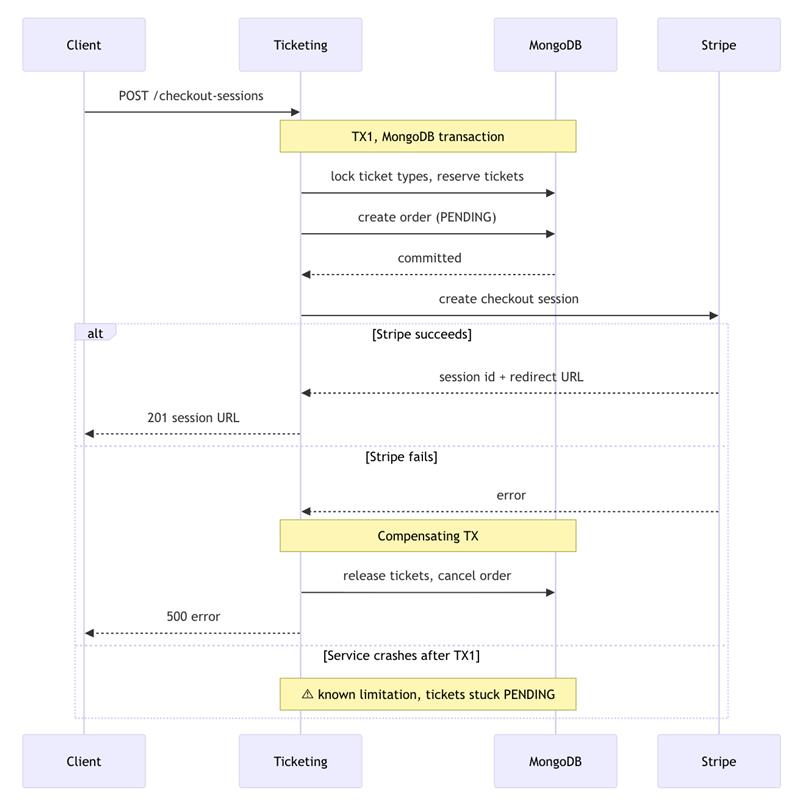
\includegraphics[width=\textwidth]{../public/implementation/saga.jpeg}
  \caption{Ticket purchase saga sequence diagram}
  \label{fig:saga}
\end{figure}

\subsection{Service Architecture Patterns}

Services adopt different internal architectural styles.

\paragraph{Clean Architecture (\texttt{ticketing}, \texttt{user}, \texttt{event}, \texttt{notification}).}
Some services are structured around \textbf{Clean Architecture} with \textbf{Domain-Driven Design} principles. The codebase is organised into four layers with strict inward dependency rules:

\begin{itemize}
  \item \texttt{domain/}: contains aggregates, value objects, domain events, repository interfaces and domain service interfaces. No dependency on any framework or infrastructure.
  \item \texttt{application/}: contains use cases, application services and DTOs. Orchestrates domain logic without touching infrastructure directly.
  \item \texttt{infrastructure/}: contains concrete implementations of repository interfaces (MongoDB), external service adapters (Stripe, Keycloak), mappers between domain objects and persistence schemas.
  \item \texttt{presentation/}: contains HTTP controllers, RabbitMQ consumers and WebSocket gateways. Translates inbound requests into application-layer calls.
\end{itemize}

This separation ensures that domain logic is fully isolated from infrastructure concerns and it's independently testable. Within this structure, the organization of the application layer varies by service: \texttt{event} and \texttt{notification} use \textbf{Command Query Responsibility Segregation} (CQRS) pattern, with write operations represented as commands and read operations as queries, each handled by a dedicated class. The remaining services use a unified application service or handler approach without explicit read/write separation. The current implementation uses a single shared data model for reads and writes; fully separating the read and write models would unlock further performance and scalability gains and is a natural evolution of the current design.

\paragraph{NestJS module organisation (\texttt{chat}, \texttt{interaction}).}
Some services adopt the \textbf{NestJS default module structure}: the codebase is organised by feature module (e.g. \texttt{conversations}, \texttt{users} in \texttt{chat}), each encapsulating its own controllers, services and Mongoose schemas.

\newpage
\section{Validation}

The system has been validated through a combination of automated testing and API-level verification, with the objective of verifying both the internal correctness of services and the proper behavior of exposed interfaces.

Two main testing approaches have been adopted: unit and integration testing of service logic, and API-level testing through interactive documentation.

\subsection{Automated Testing and Coverage}

Each service has been tested through automated tests designed to cover:
\begin{itemize}
  \item domain logic and service-layer behavior;
  \item validation rules and edge cases.
\end{itemize}

Integration tests of data persistence operations have been performed using a MongoDB in-memory implementation or by a MongoDB container automatically started (and torn down) during Gradle test execution.

To assess the effectiveness of the test suite, code coverage has been measured. The project achieves an overall coverage of at least 70\%, ensuring that the majority of the codebase is exercised during testing. This level of coverage provides reasonable confidence in the correctness of the implemented logic.

\subsection{API Testing}

In addition to automated tests, the system has been validated through direct interaction with the exposed APIs.

Each service provides a formal API specification compliant with the OpenAPI standard, which allows endpoints to be explored and tested interactively. This interface has been used to manually verify the correctness of request handling, response formats and error management.

API testing has been particularly useful for:
\begin{itemize}
  \item validating request/response workflows;
  \item testing edge cases and invalid inputs;
  \item verifying correctness of response formats.
\end{itemize}

The full set of APIs is available at: \url{https://eventonight.github.io/EvenToNight/openAPI/}.

Moreover, APIs have been tested in integration with the frontend, ensuring correct implementation and usage.

\newpage
\section{Deployment Instructions}

The application supports two deployment modes: \textbf{Docker Compose} for single-node setups and \textbf{Docker Swarm} (beta) for multi-node, highly available deployments. In both cases, all services run as independent containers and are managed via a centralised script.

\subsection{Installation}

\noindent\textbf{1. Clone the repository.}\par
\begin{lstlisting}[language=bash]
git clone https://github.com/EvenToNight/EvenToNight.git
cd EvenToNight
\end{lstlisting}

\noindent\textbf{2. Configure environment variables.}\par
\begin{lstlisting}[language=bash]
cp .env.template .env
# Edit .env and fill in all required fields
# Note: if using the --no-deps flag, Stripe keys can contain arbitrary values. All fields must still be filled in.
\end{lstlisting}

\subsection{Docker Compose}

\noindent\textbf{Option A: Use pre-built images from ghcr.io (Recommended).}\par
\begin{lstlisting}[language=bash]
# Pull images
./scripts/composeApplication.sh pull

# Pull images with database seeding
./scripts/composeApplication.sh --init-db pull

# Deploy the application
./scripts/composeApplication.sh up -d --wait

# Deploy with database seeding
./scripts/composeApplication.sh --init-db up -d --wait

# Deploy in development mode (with host-mapped ports and dashboards for databases, RabbitMQ and Traefik)
./scripts/composeApplication.sh --init-db --dev up -d --wait
\end{lstlisting}

\noindent\textbf{Option B: Local build.}
Add the \texttt{-{}-build} flag to build services locally instead of using pre-built images. The \texttt{-{}-dev} flag is required as it includes the build instructions:
\begin{lstlisting}[language=bash]
# Build and deploy
./scripts/composeApplication.sh --dev up --build -d --wait

# Build and deploy with seeding
./scripts/composeApplication.sh --init-db --dev up --build -d --wait
\end{lstlisting}

\noindent\textbf{Additional flags.}\par\noindent
\texttt{-{}-no-deps}: Excludes external dependencies (Stripe). The flag can be added to any deploy command to exclude external services:
\begin{lstlisting}[language=bash]
# Deploy without external dependencies
./scripts/composeApplication.sh --no-deps up -d --wait

# Deploy with seeding but without external dependencies
./scripts/composeApplication.sh --init-db --no-deps up -d --wait
\end{lstlisting}

\noindent \textbf{Note:} When using \texttt{-{}-no-deps}, the Stripe keys (\texttt{STRIPE\_SECRET\_KEY}, \texttt{STRIPE\_PUBLISHABLE\_KEY}, \texttt{STRIPE\_WEBHOOK\_SECRET}) in \texttt{.env} can contain arbitrary values.

\noindent\texttt{-{}-project-name}: Overrides the Docker Compose project name (defaults to \texttt{eventonight}):
\begin{lstlisting}[language=bash]
./scripts/composeApplication.sh --project-name myproject up -d --wait
\end{lstlisting}

\noindent\textbf{Stripe configuration.}\label{par:stripe-config} For Stripe payments in a local environment (required only if NOT using \texttt{-{}-no-deps}):
\begin{lstlisting}[language=bash]
./services/payments/scripts/local-webhooks.sh
\end{lstlisting}

\noindent This script must be run to forward Stripe webhooks to the local environment. For more information on using sandbox mode, refer to the \href{https://docs.stripe.com/testing}{Stripe documentation}.

\noindent\textbf{Alternative setup.} Use Gradle to set up the entire environment with seeding and the Stripe listener:
\begin{lstlisting}[language=bash]
./gradlew setupApplicationEnvironment
\end{lstlisting}

\noindent\textbf{Teardown.}\par
\begin{lstlisting}[language=bash]
./scripts/composeApplication.sh down
./scripts/composeApplication.sh down -v   # also remove volumes
./gradlew teardownApplicationEnvironment  # via Gradle
\end{lstlisting}

\subsection{Docker Swarm (Beta)}

\noindent\textbf{Prerequisites.}\par
Initialise the swarm on the manager node:
\begin{lstlisting}[language=bash]
docker swarm init
\end{lstlisting}

\noindent Join additional worker nodes using the token provided by the manager:
\begin{lstlisting}[language=bash]
docker swarm join --token <token> <manager-ip>:2377
\end{lstlisting}

\noindent\textbf{Option A: Use pre-built images from ghcr.io (Recommended).}\par
\begin{lstlisting}[language=bash]
./scripts/deploySwarm.sh
\end{lstlisting}

\noindent The \texttt{-{}-auto-labels} flag can be added to automatically assign placement labels to nodes in a balanced way, without having to configure them manually:
\begin{lstlisting}[language=bash]
./scripts/deploySwarm.sh --auto-labels
\end{lstlisting}

\noindent\textbf{Note:} On the first deploy, database seeding is performed automatically.

\newpage
\noindent\textbf{Option B: Local build.}\par
Build images locally and push them to Docker Hub (multi-arch) so all workers have access to them, then deploy:
\begin{lstlisting}[language=bash]
./scripts/deploySwarm.sh --local --build
\end{lstlisting}

\noindent To override the hostname baked into the frontend image (defaults to \texttt{HOST} from \texttt{.env}, e.g. to use \texttt{localhost} for local testing):
\begin{lstlisting}[language=bash]
./scripts/deploySwarm.sh --local --build --host <hostname> --auto-labels
\end{lstlisting}

\noindent To deploy using already-pushed local images (without rebuilding):
\begin{lstlisting}[language=bash]
./scripts/deploySwarm.sh --local
\end{lstlisting}

\noindent To build and push without deploying:
\begin{lstlisting}[language=bash]
./scripts/deploySwarm.sh --build
\end{lstlisting}

\noindent\textbf{Additional flags.}\par\noindent
\texttt{-{}-no-deps}: Same behaviour as in Docker Compose: excludes external dependencies. Stripe configuration applies equally (see p.~\pageref{par:stripe-config}).
\begin{lstlisting}[language=bash]
./scripts/deploySwarm.sh --no-deps
\end{lstlisting}

\noindent\texttt{-{}-stack-name}: Overrides the stack name (defaults to \texttt{eventonight-swarm}):
\begin{lstlisting}[language=bash]
./scripts/deploySwarm.sh --stack-name mystack
\end{lstlisting}

\noindent\textbf{Recovery.}\par
If some services are not fully running after a deploy, the recovery script force-updates only the failing ones:
\begin{lstlisting}[language=bash]
./scripts/swarmRecover.sh [STACK_NAME]
\end{lstlisting}

\noindent To check the current status of all services without recovering:
\begin{lstlisting}[language=bash]
./scripts/swarmRecover.sh [STACK_NAME] --status
\end{lstlisting}

\noindent \texttt{STACK\_NAME} defaults to \texttt{eventonight-swarm}.

\noindent\textbf{Teardown.}\par
\begin{lstlisting}[language=bash]
./scripts/deploySwarm.sh --stop
./scripts/deploySwarm.sh --stop --remove-volumes
./scripts/deploySwarm.sh --remove-local-images  # remove test images from Docker Hub
\end{lstlisting}

Alternatively, the application is already running in production at \href{https://eventonight.site/it}{EvenToNight}.

\newpage
\section{Usage Examples}

Below are some examples of interaction with the application, illustrating the main usage flows.

Specifically, the following use cases are shown:

\begin{itemize}
  \item \textbf{Explore the platform}
  \item \textbf{Login and Registration}
  \item \textbf{Create an event}
  \item \textbf{Attend an event}
  \item \textbf{Review an event}
  \item \textbf{Contact an organization}
\end{itemize}

The storyboards are presented directly using the developed platform, showing the main user interactions.

In the examples below, some secondary or repetitive navigation dynamics have been omitted.

\subsection{Explore the Platform}

A user who opens the platform can start exploring it. In particular, they can discover proposed events or search for them directly via the search bar. If they want to see more results, they can go to a dedicated page for exploring the platform content, where it is possible to filter events and more conveniently search for users and organizations.

\begin{figure}[H]
  \centering
  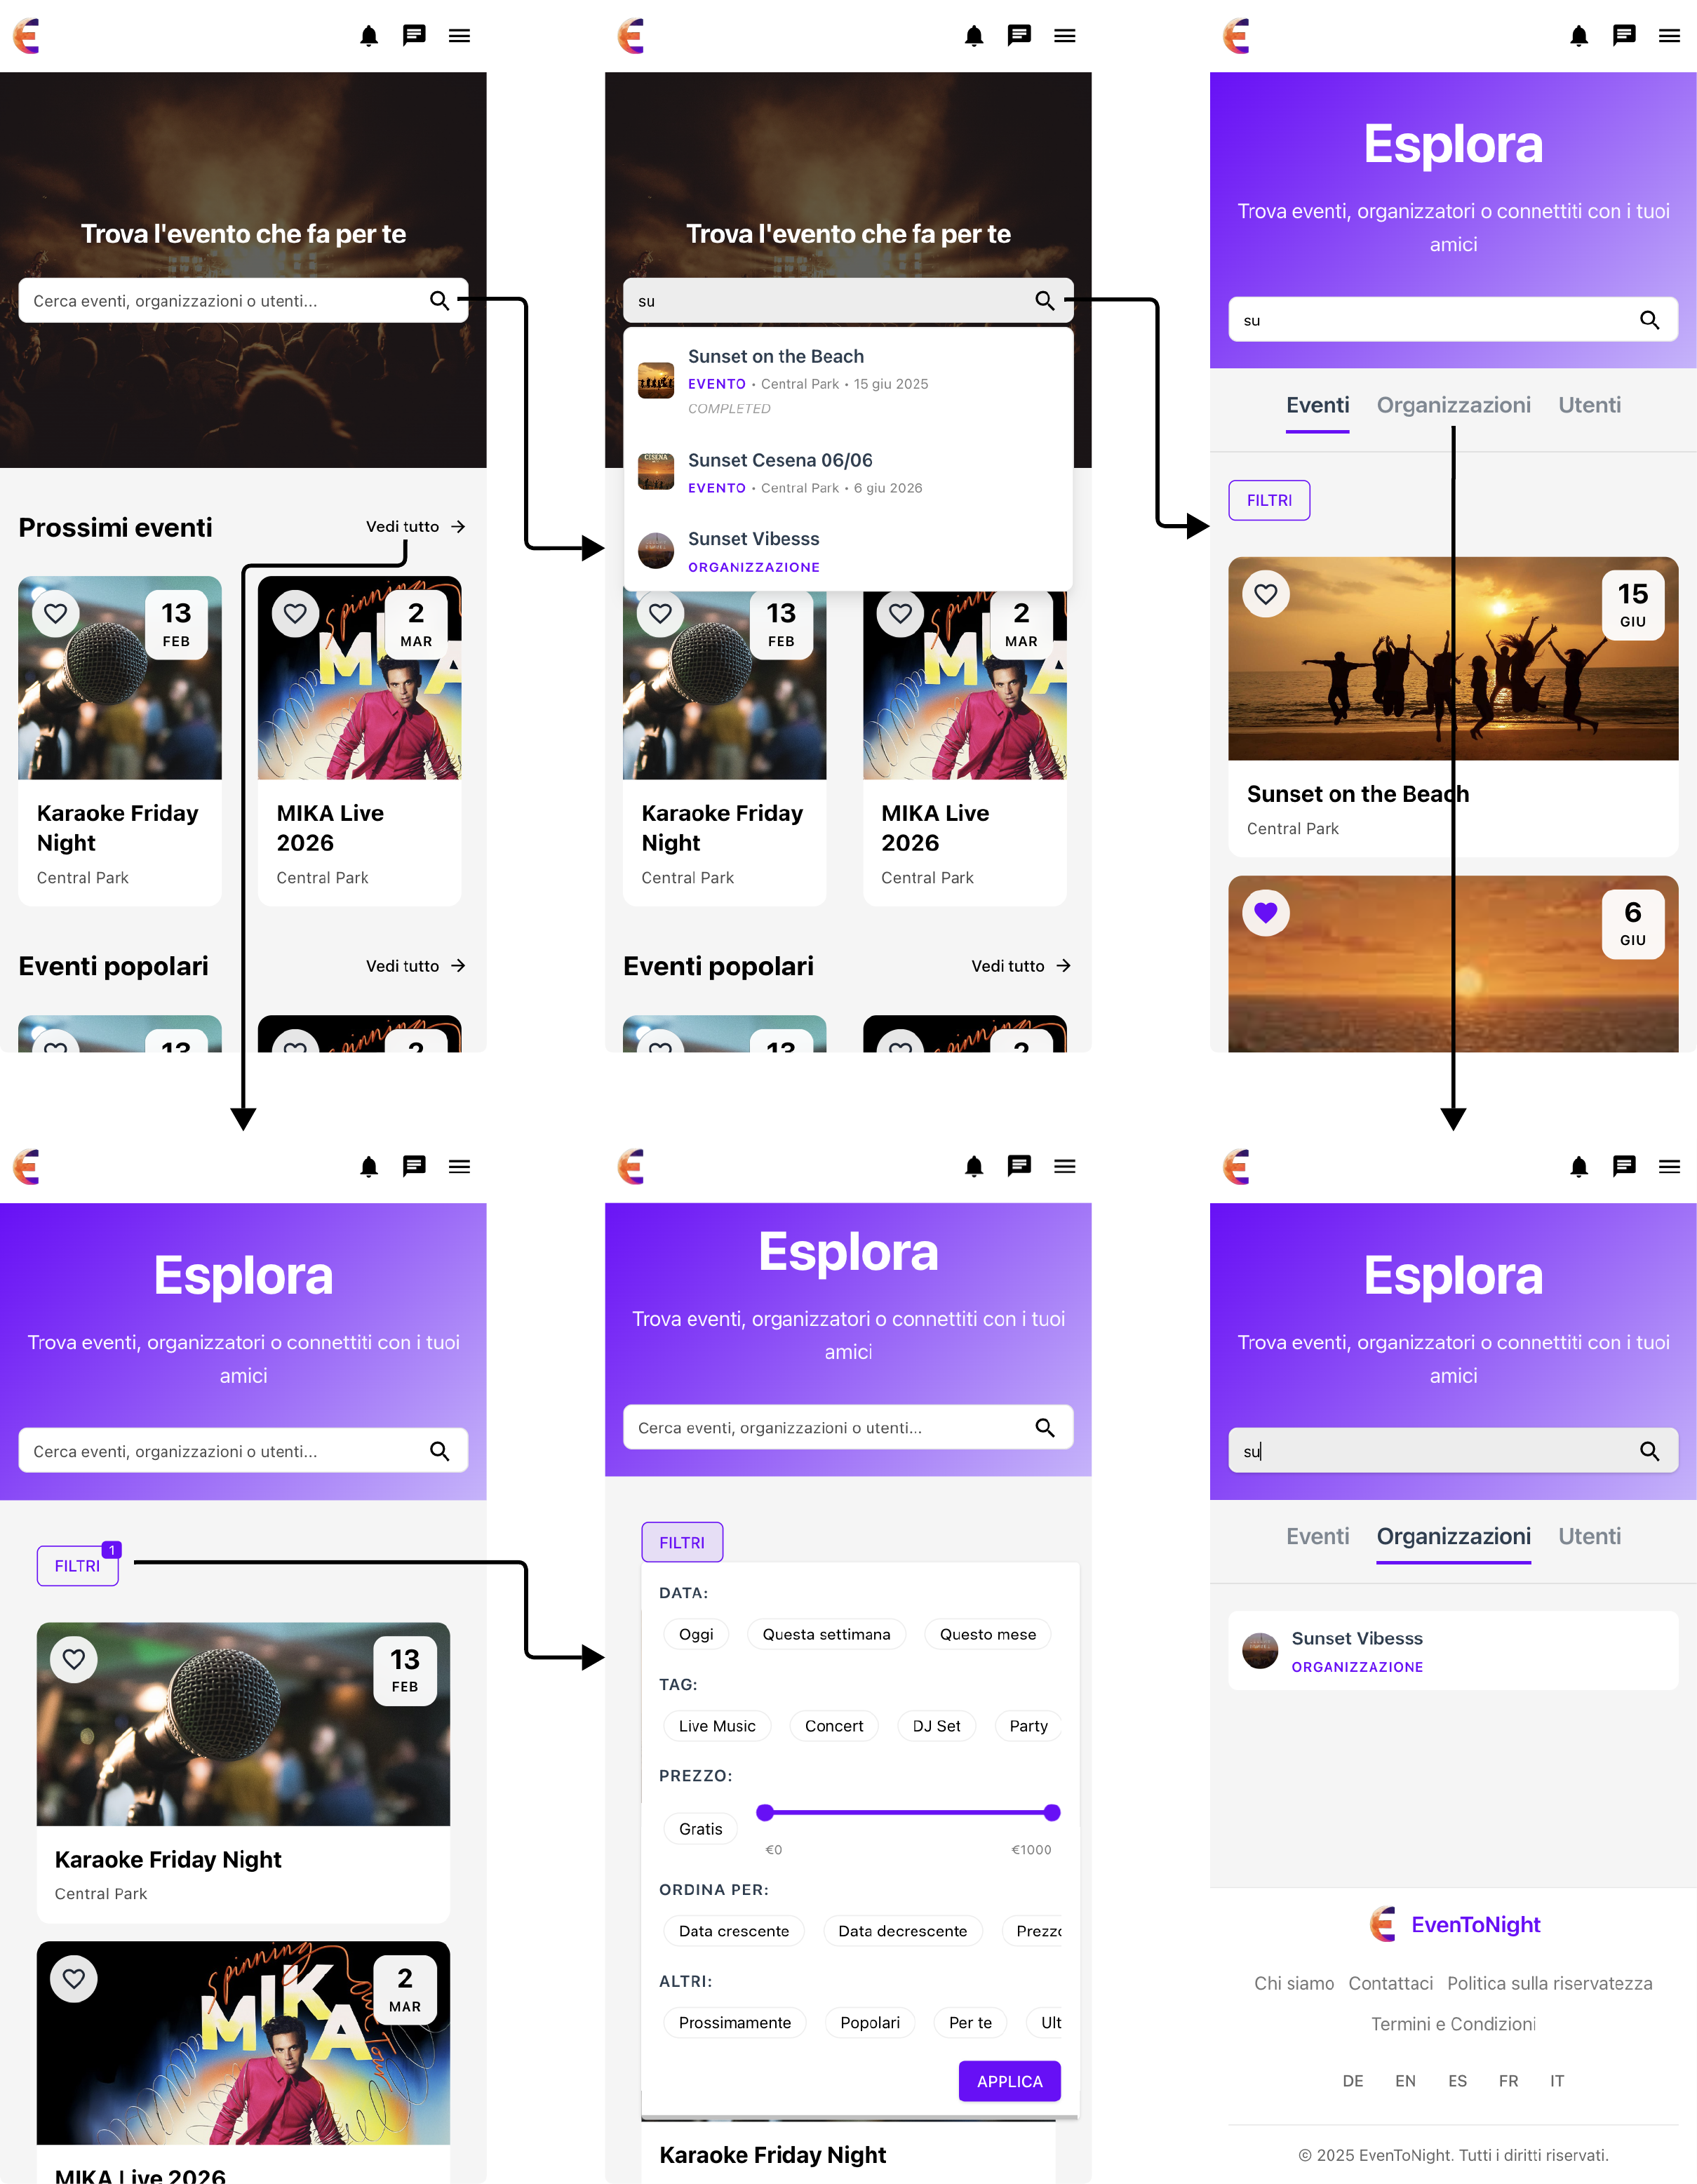
\includegraphics[width=\textwidth]{../public/storyboard/Storyboard-Explore.png}
  \caption{Storyboard: Exploring the platform}
  \label{fig:storyboard-explore}
\end{figure}

\subsection{Login and Registration}

After opening the application, a user can log in or register to access the additional features offered by the platform.

\begin{figure}[H]
  \centering
  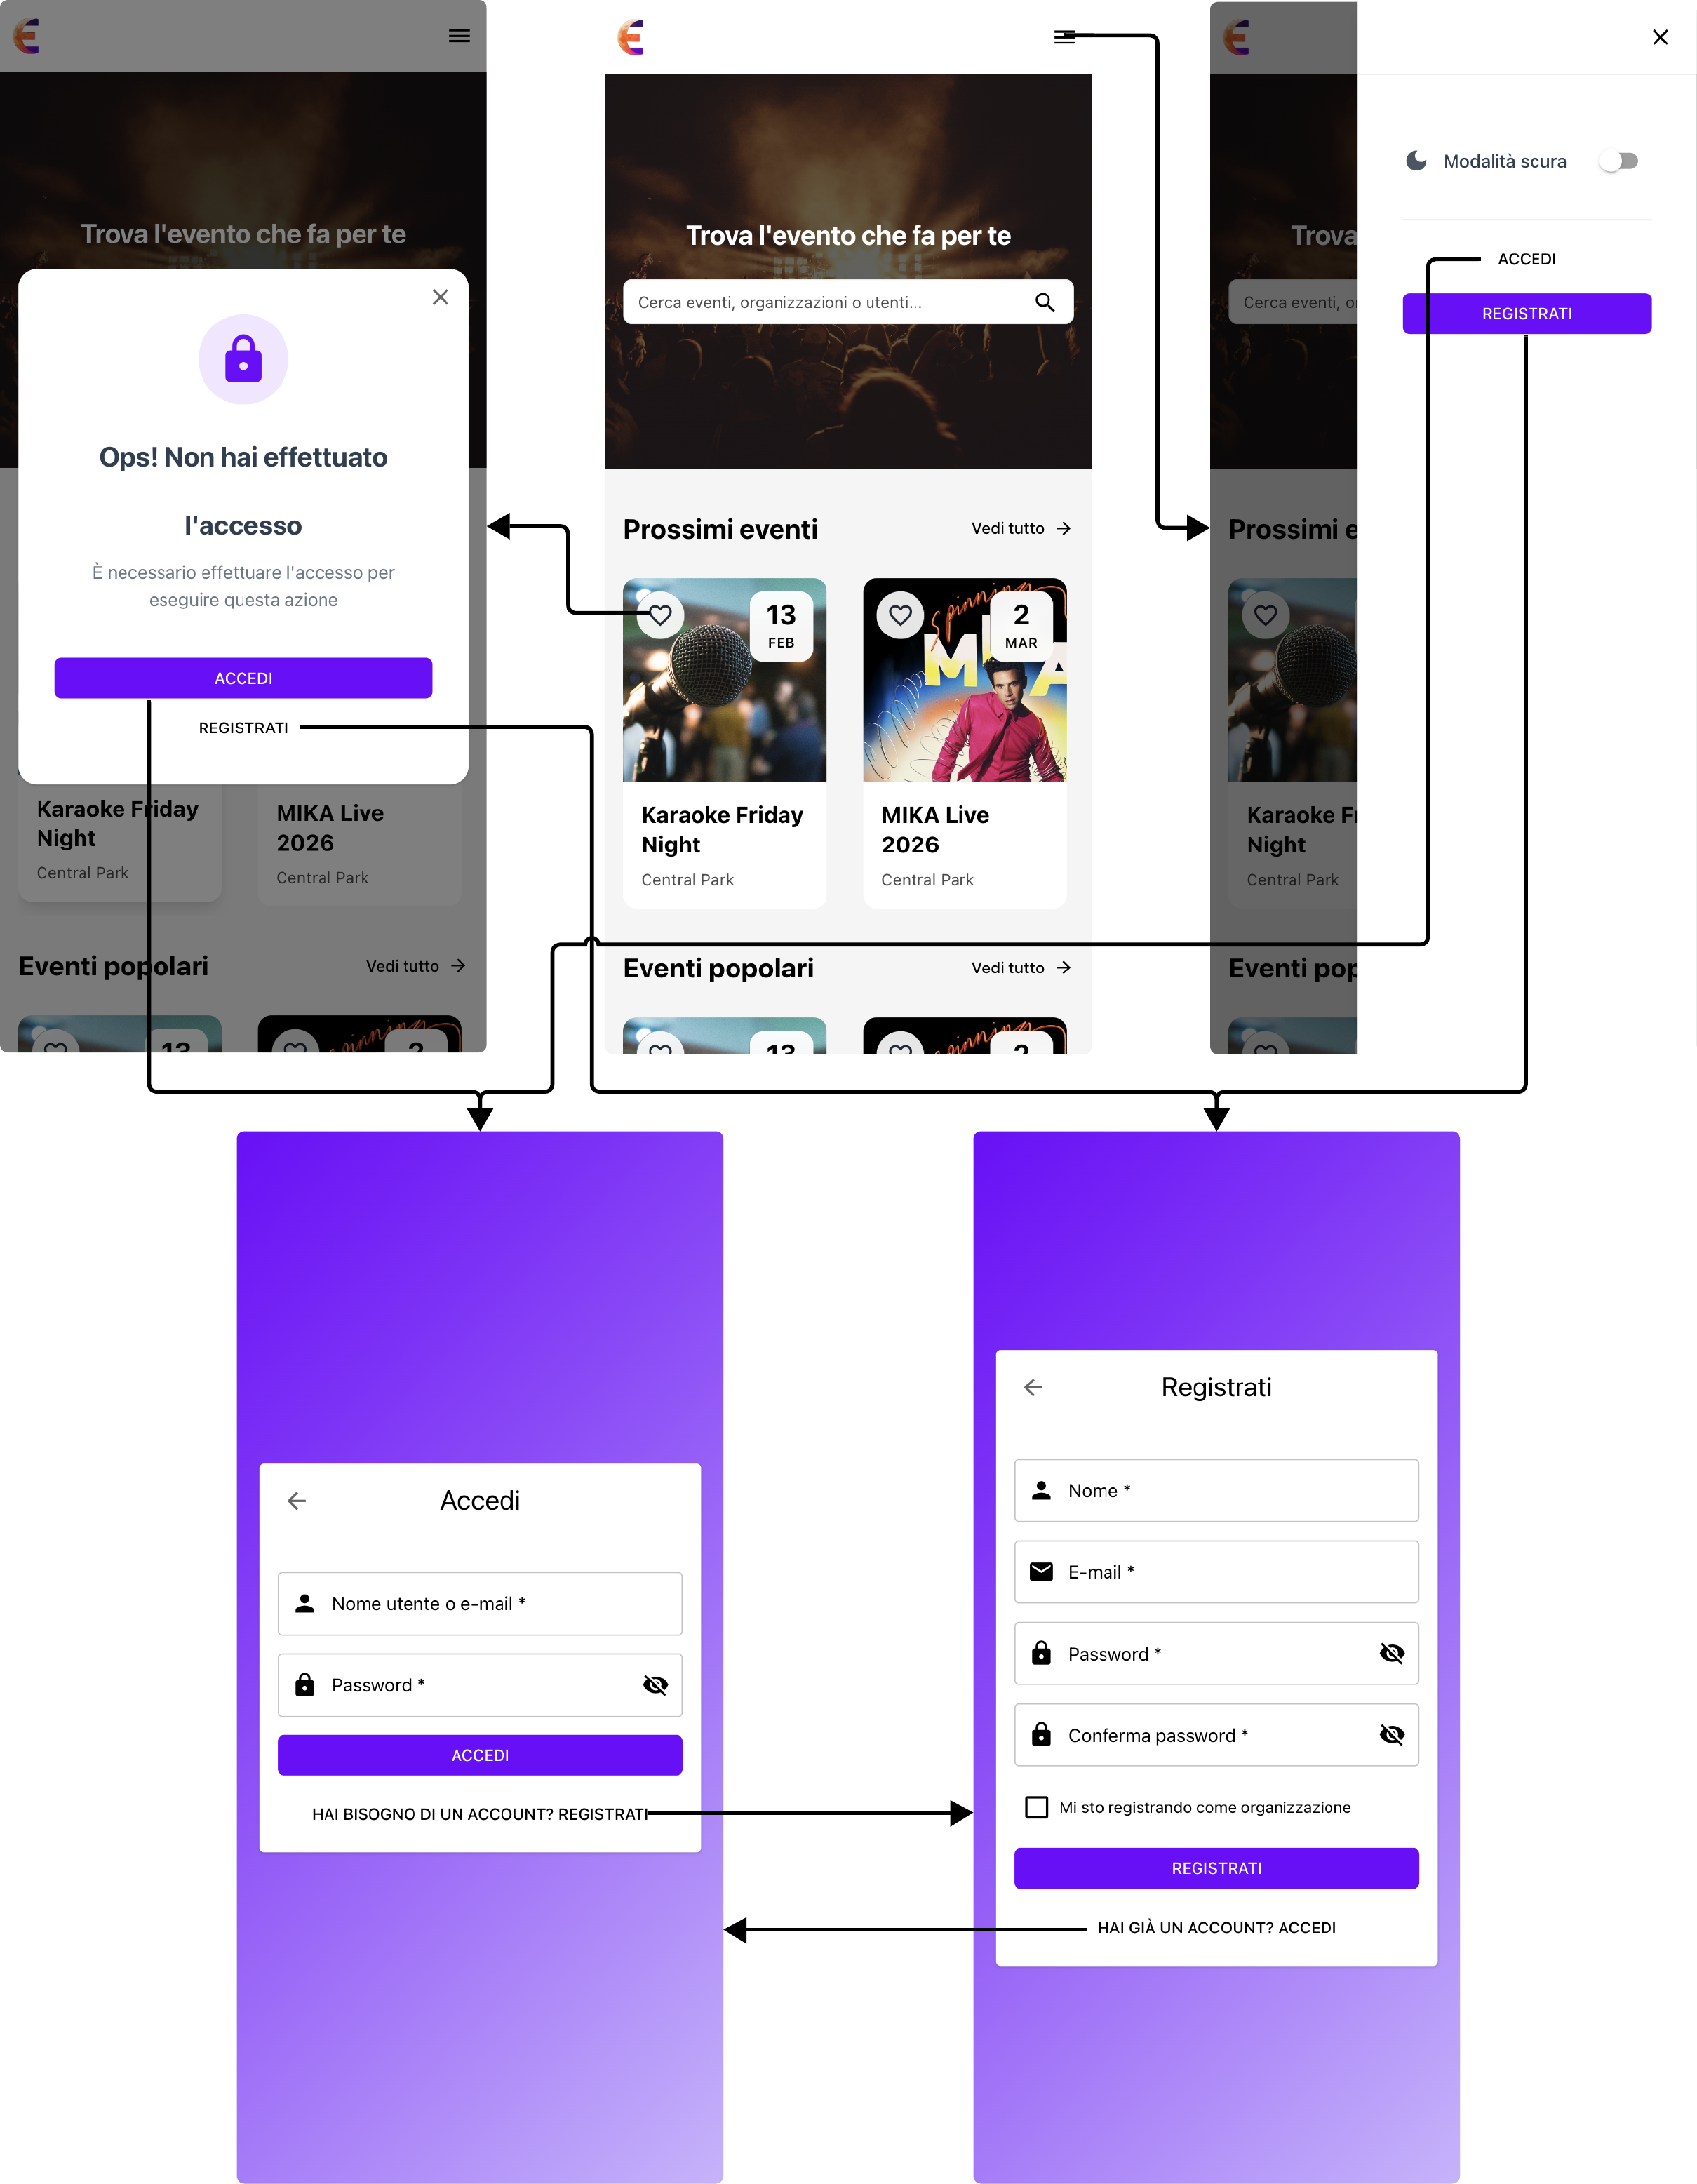
\includegraphics[width=\textwidth]{../public/storyboard/Storyboard-Login.png}
  \caption{Storyboard: Login and registration}
  \label{fig:storyboard-login}
\end{figure}

\subsection{Create an Event}

An organization that has registered on the platform can create events. The creation happens through a form where all the relevant data is entered. It is also possible to temporarily create a draft of the event and continue editing it later.

\begin{figure}[H]
  \centering
  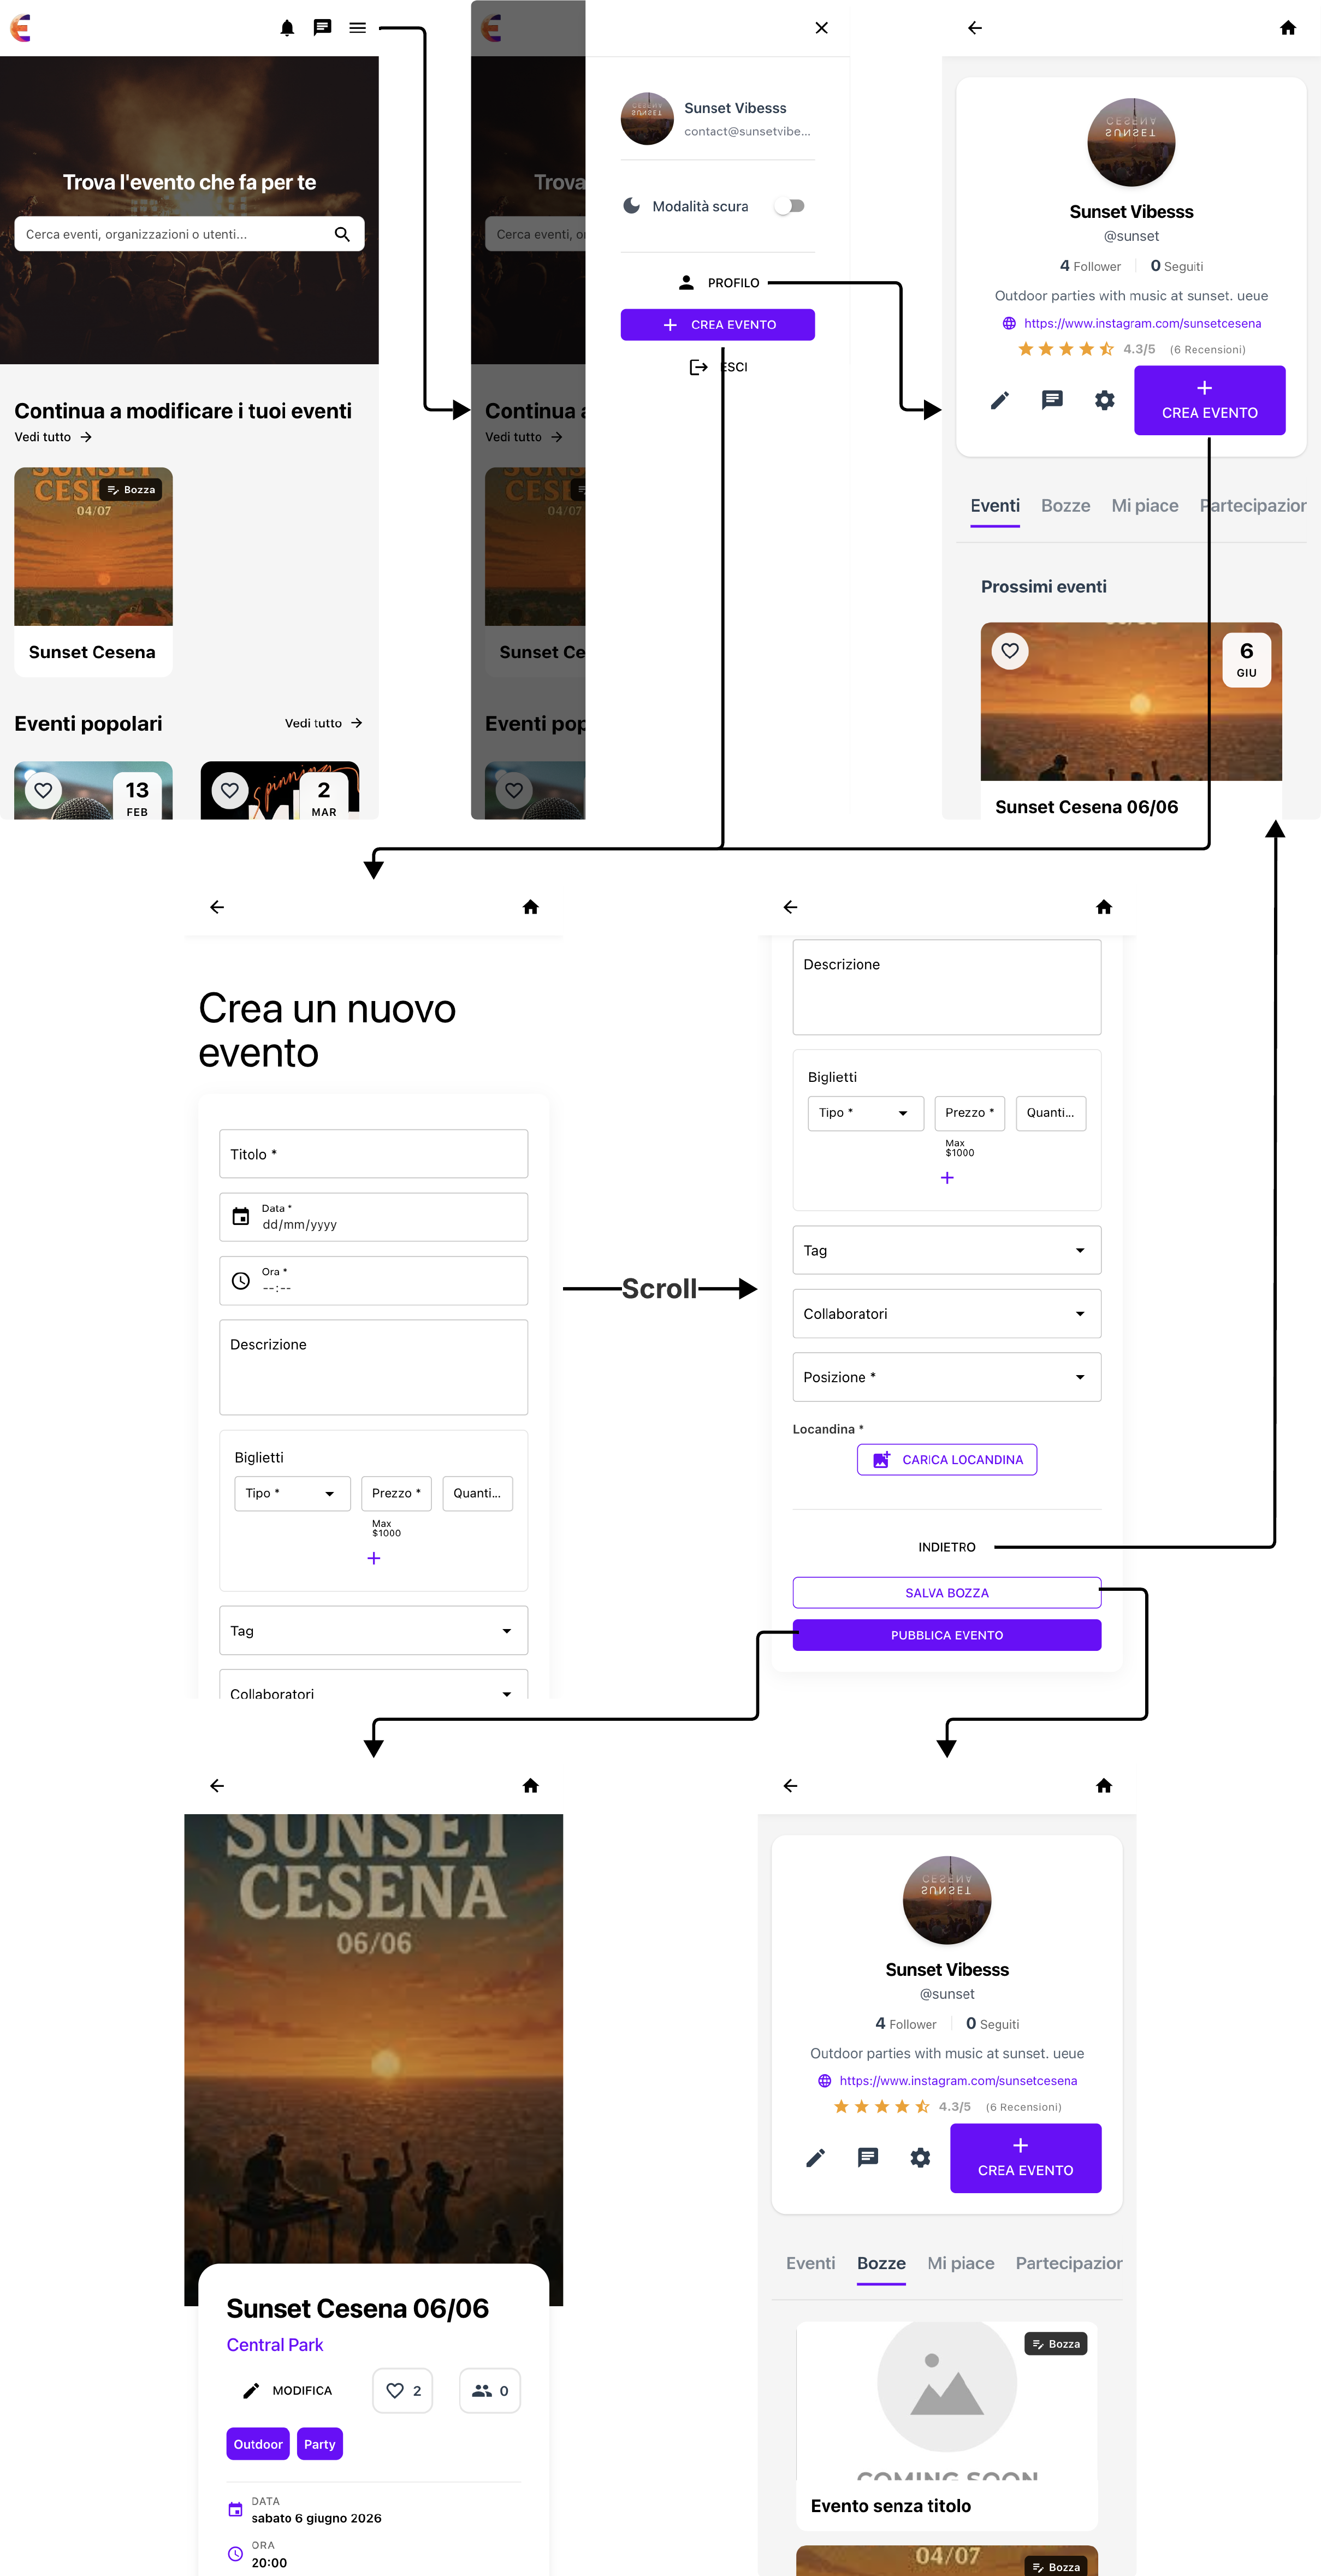
\includegraphics[width=0.75\textwidth]{../public/storyboard/Storyboard-Create-Event.png}
  \caption{Storyboard: Creating an event}
  \label{fig:storyboard-create-event}
\end{figure}

\subsection{Attend an Event}

A registered user can purchase tickets for different events and view them later. The tickets will contain a QR code that organizations can use to verify them.

\begin{figure}[H]
  \centering
  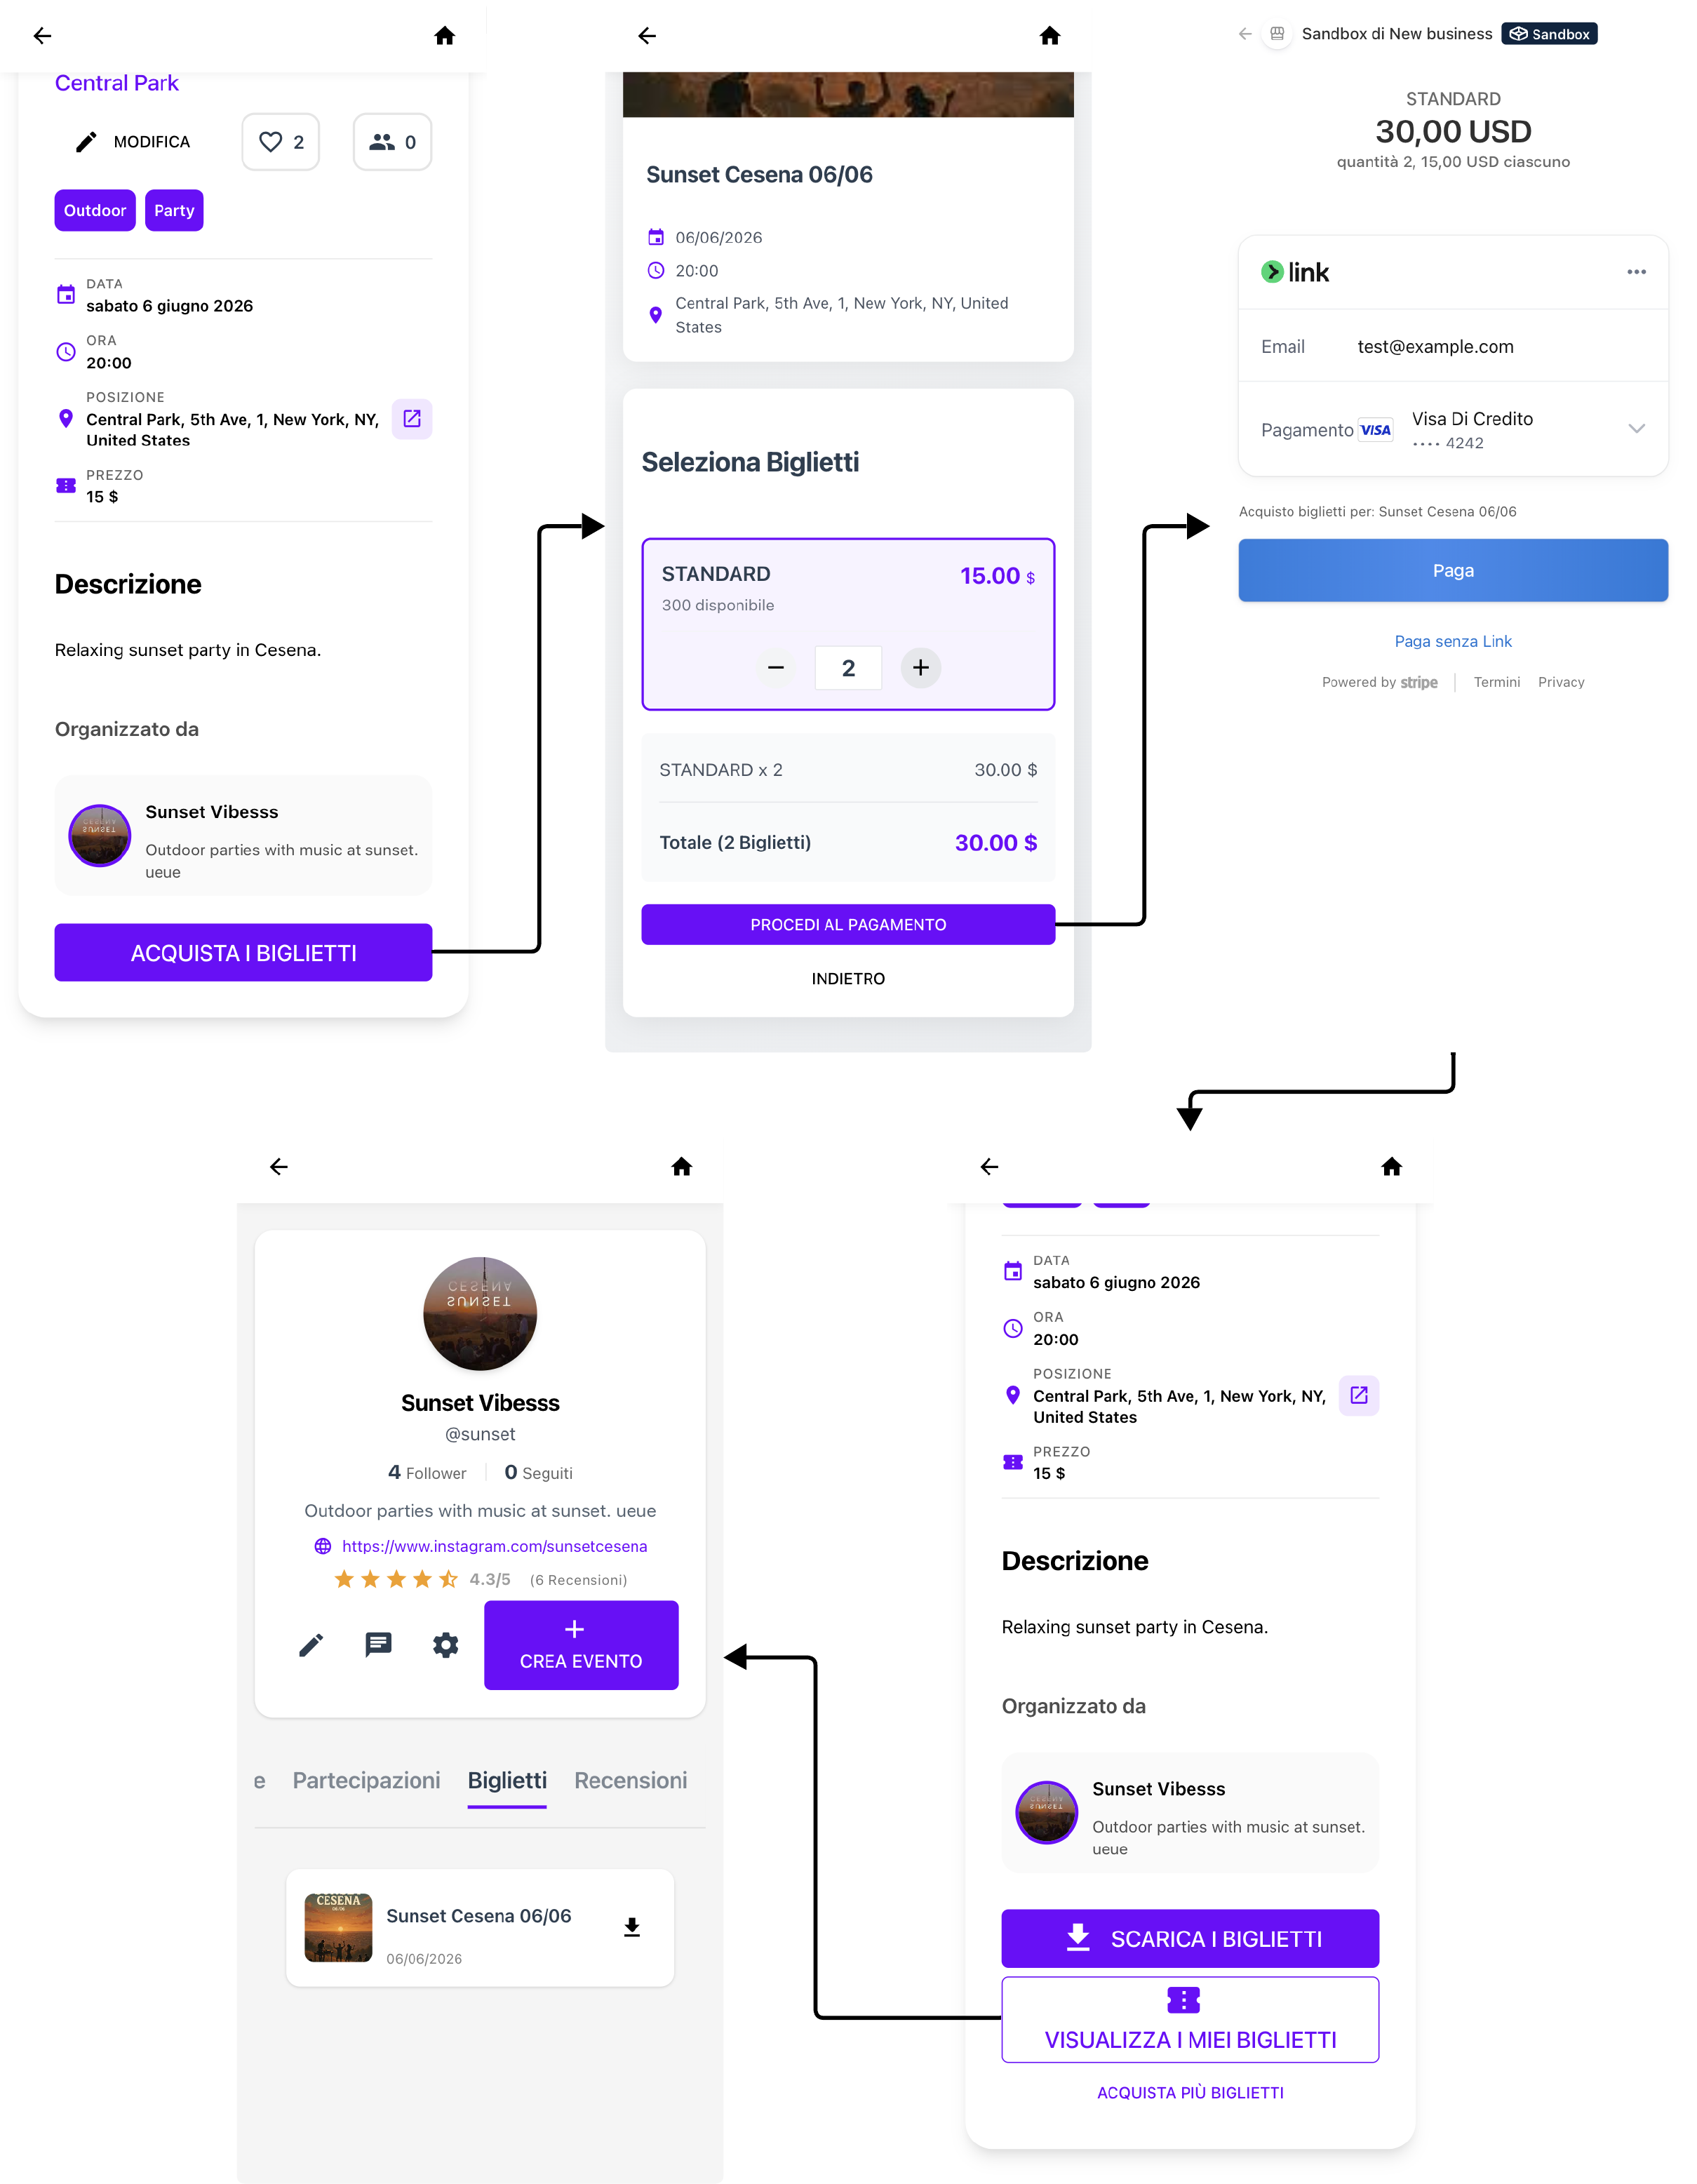
\includegraphics[width=\textwidth]{../public/storyboard/Storyboard-Buy-Ticket.png}
  \caption{Storyboard: Purchasing a ticket}
  \label{fig:storyboard-buy-ticket}
\end{figure}

\subsection{Review an Event}

After attending an event, a user can decide to leave a review. Once submitted, they cannot leave another review for the same event, but they can modify or delete it.

\begin{figure}[H]
  \centering
  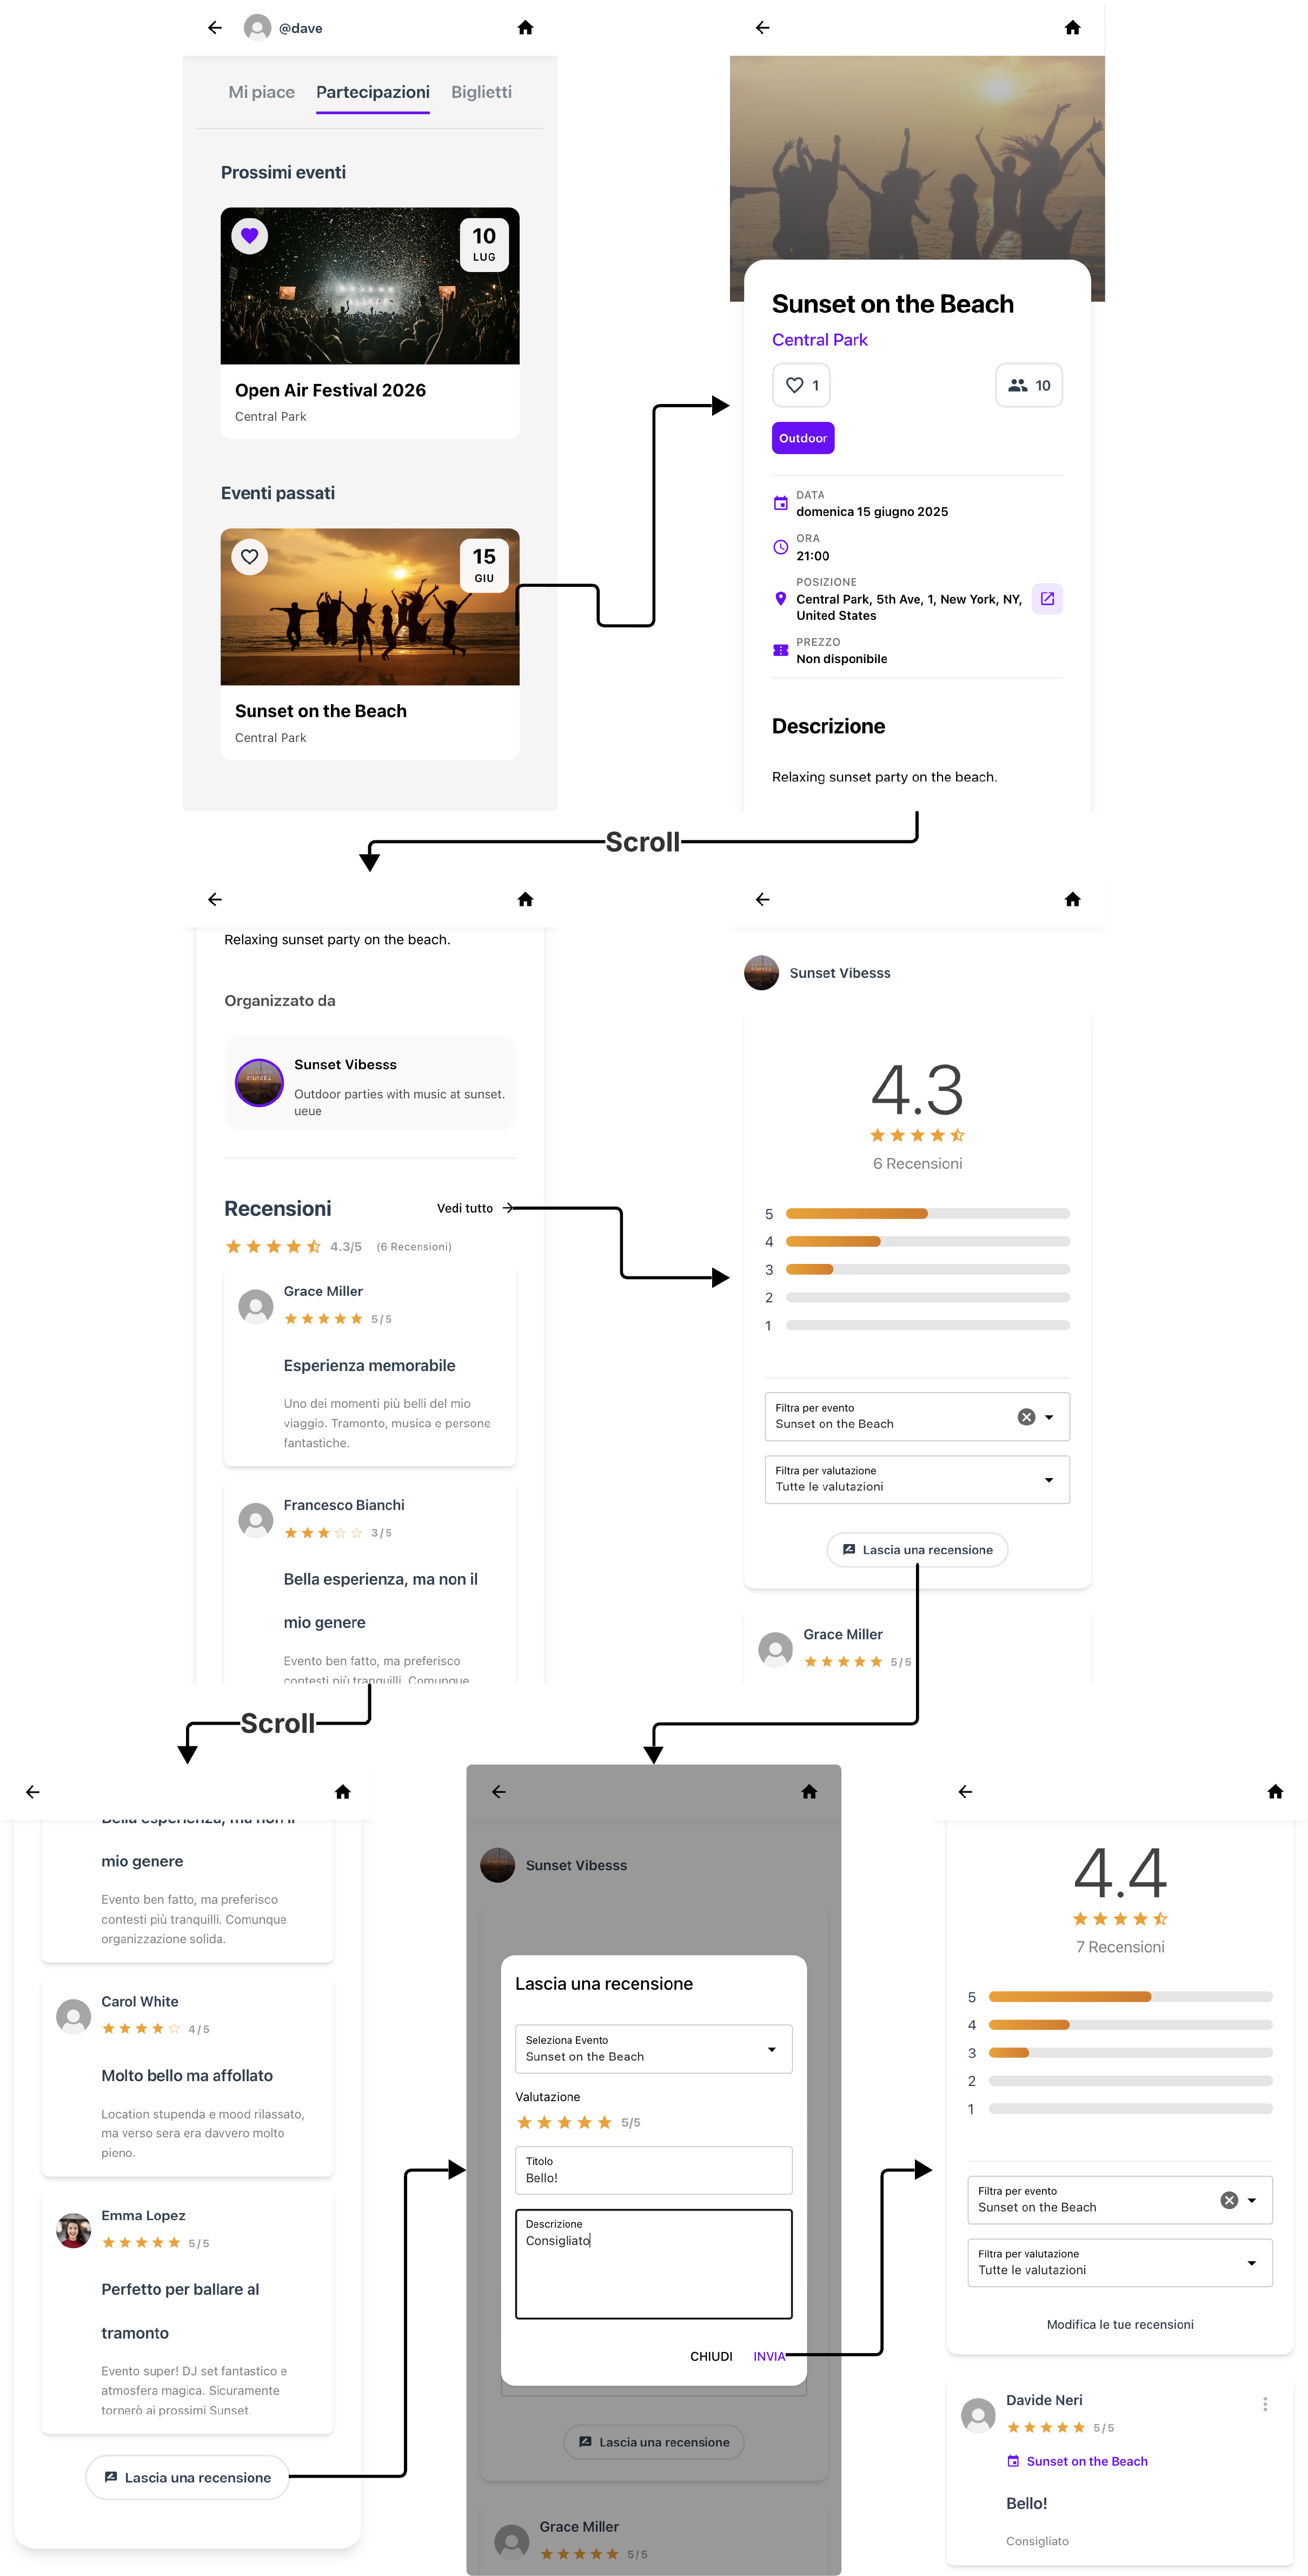
\includegraphics[width=0.65\textwidth]{../public/storyboard/Storyboard-Reviews.png}
  \caption{Storyboard: Reviewing an event}
  \label{fig:storyboard-reviews}
\end{figure}

\subsection{Contact an Organization}

A registered user may need to contact an organization to ask for more information or for potential issues.

\begin{figure}[H]
  \centering
  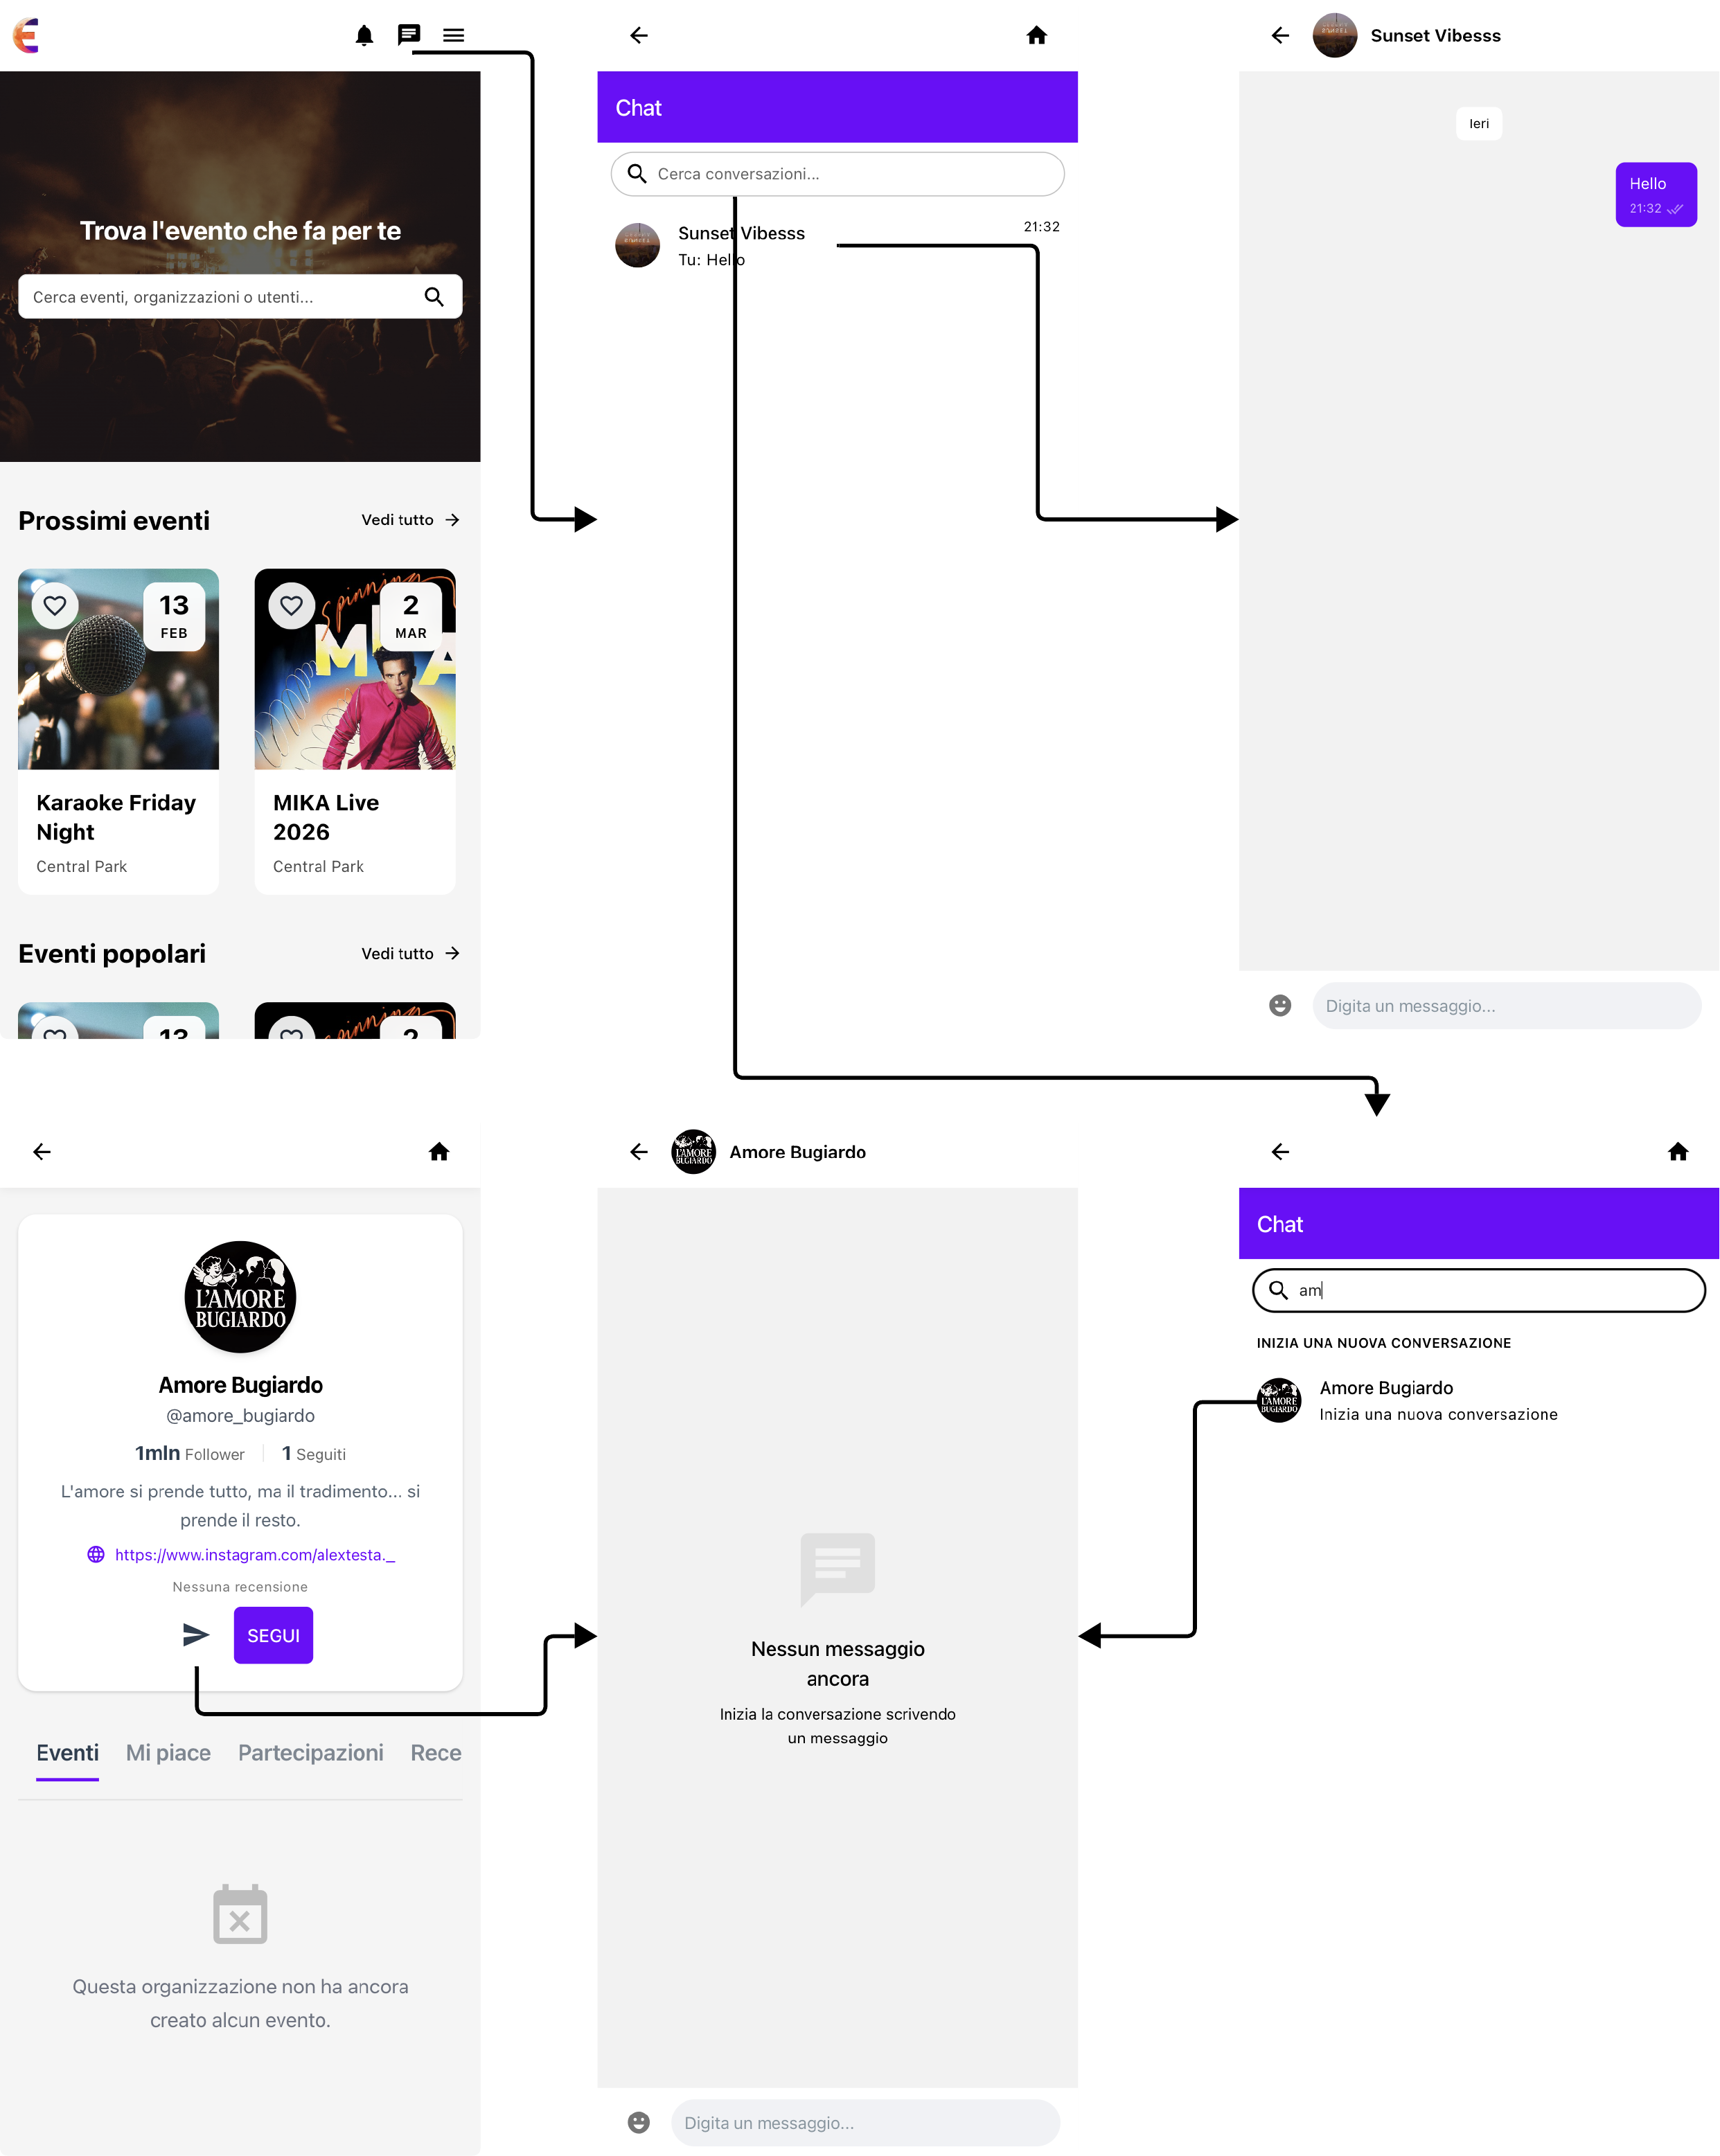
\includegraphics[width=\textwidth]{../public/storyboard/Storyboard-Chat.png}
  \caption{Storyboard: Contacting an organization}
  \label{fig:storyboard-chat}
\end{figure}

\newpage
\section{Conclusions}

We are satisfied with the platform developed, which originated from our business idea. The main achievements are:

\begin{itemize}
  \item \textbf{Achievement of project goals.} All project goals were reached, with particular focus on aspects defining a distributed system. The system consists of isolated, loosely coupled components that appear to users as a single coherent platform.

  \item \textbf{Requirements fulfillment.} All functional and non-functional requirements were satisfied, with iterative refinement based on feedback from potential users.

  \item \textbf{Microservices architecture design.} The system was designed as a collection of independent services with clear boundaries. Backend microservices communicate and coordinate via a message broker and expose well-defined REST APIs used by the frontend.

  \item \textbf{Distributed architecture implementation.} Services were containerized using Docker and deployed both with Docker Compose and Docker Swarm, simulating a distributed environment with service isolation and internal networking.

  \item \textbf{Modularity and extensibility.} The architecture provides a clear separation of concerns, ensuring maintainability, easy addition of new features and future scalability. The modular design also facilitated parallel development of different functionalities.
\end{itemize}

\subsection{Future Works}

Although the platform was designed according to distributed principles, it was deployed on a single physical machine. As a result, the system does not provide real high availability: if the host machine fails, all services become unavailable. Future improvements could include deployment on multiple physical or virtual machines to achieve infrastructure-level fault tolerance and resilience.

From a functional perspective, potential extensions include:

\begin{itemize}
  \item Allowing organizations to respond to reviews.
  \item Additional notifications, such as friendship suggestions and updates on liked events.
  \item Profile insights and statistics.
  \item Refund management.
  \item Multi-currency support to enhance internationalization.
\end{itemize}

\subsection{What We Learned}

This project allowed us to apply distributed system concepts that we had previously studied only from a theoretical perspective. In particular:

\begin{itemize}
  \item We gained practical experience with the trade-offs between consistency and availability in the presence of network partitions, as described by the CAP theorem.

  \item We experimented with containerization and faced challenges in guaranteeing data consistency across multiple services and system correctness when multiple replicas are deployed.

  \item We gained a deeper understanding of service decoupling, transparency, reliability and resilience both in single and multiple node deployments.

  \item We learnt how to make a real online deployment using a proprietary domain and physical server.
\end{itemize}


\end{document}
